\documentclass[twoside,12pt]{book}
\usepackage[top=2.5cm, bottom=2.5cm, outer=2cm, inner=3cm, headsep=14pt]{geometry}

\usepackage{kantlipsum}
\usepackage{fancyhdr}
\fancyhf{} % clear all header and footers
\renewcommand{\headrulewidth}{0pt} % remove the header rule
\fancyfoot[LE,RO]{\thepage} % Left side on Even pages; Right side on Odd pages
\pagestyle{fancy}
\fancypagestyle{plain}{%
  \fancyhf{}%
  \renewcommand{\headrulewidth}{0pt}%
  \fancyhf[lef,rof]{\thepage}%
}

% \usepackage{pdfpages}
\usepackage{textpos}
\usepackage{times}
\usepackage[utf8x]{inputenc}
\usepackage[T1]{fontenc}
\usepackage{polski}
\usepackage{setspace}
\usepackage{color}
\usepackage{graphicx}
\usepackage{url}
\usepackage[usenames,dvipsnames,svgnames]{xcolor}
\usepackage{graphbox}
\usepackage{tikz}
\usepackage{varwidth}

\usepackage{lipsum}
%\usepackage{caption}
\usepackage{fancyhdr}
\usepackage{pgf}
\usepackage{pgfpages}
\usepackage{wrapfig}
\usepackage{textcomp}

\usepackage{longtable}
\usepackage{booktabs}
\usepackage{ltablex}
\usepackage{multirow}
\usepackage{afterpage}
\newcommand\blankpage{%
    \null
    \thispagestyle{empty}%
    \addtocounter{page}{-1}%
    \newpage}

\renewcommand{\baselinestretch}{1.15}
%listingi
\usepackage{listings}
\lstset{
    language=bash,
    basicstyle=\ttfamily\small,
    aboveskip={1.0\baselineskip},
    belowskip={1.0\baselineskip},
    columns=fixed,
    extendedchars=true,
    breaklines=true,
    tabsize=2,
    prebreak=\raisebox{0ex}[0ex][0ex]{\ensuremath{\hookleftarrow}},
    frame=lines,
    showtabs=false,
    showspaces=false,
    showstringspaces=false,
    keywordstyle=\color[rgb]{0.627,0.126,0.941},
    commentstyle=\color[rgb]{0.133,0.545,0.133},
    stringstyle=\color[rgb]{01,0,0},
    numbers=left,
    numberstyle=\small,
    stepnumber=1,
    numbersep=7pt,
    captionpos=t,
    escapeinside={\%*}{*)}
}



%opening
\title{MSc tba}
\author{Marcin Skwarek}
\makeatletter
\def\@makechapterhead#1{%
  \vspace*{50\p@}%
  {\parindent \z@ \raggedright \normalfont
    \ifnum \c@secnumdepth >\m@ne
      \if@mainmatter
        %\huge\bfseries \@chapapp\space \thechapter
        \Huge\bfseries \thechapter.\space%
        %\par\nobreak
        %\vskip 20\p@
      \fi
    \fi
    \interlinepenalty\@M
    \Huge \bfseries #1\par\nobreak
    \vskip 40\p@
  }}
\makeatother
% \includepdf[pages=-,pagecommand={},width=\textwidth]{title.pdf}
\begin{document}
\makeatletter
\def\ps@plain{%
  \let\@mkboth\@gobbletwo
  \let\ps@normal\hf@plain
  \let\ps@opening\hf@plain
  \let\ps@closing\hf@plain
  \let\ps@blank\hf@empty
  \ps@normal}
\makeatother

% \pagestyle{plain}


% \begin{titlepage}
% \begin{center}
% 	
\includegraphics[scale=0.33]{image/weiti}
% 	%\setmainfont[Ligatures=TeX]{Helvetica}
% 	\vspace{0.7cm}
% 	\begingroup
% 	\fontsize{12pt}{12pt}\selectfont
% 		\begin{center}
% 			Instytut Telekomunikacji
% 		\end{center}
% 	\endgroup
% 	\vspace{0.7cm}
% 	
\includegraphics[scale=0.8]{image/tytul}\\
% 	\vspace{0.3cm}
% 	na kierunku telekomunikacja\\
% 	na specjalności telekomunikacja.\\
% 	\vspace{1.2cm}
% 	\begingroup
% 	\fontsize{14pt}{12pt}\selectfont
% 	\begin{center}
% 	 	\{Tytuł\}\\
% 	\end{center}
% 	\endgroup
% 	\vspace{2.3cm}
%
%
% 	\begingroup
% 	\fontsize{21pt}{12pt}\selectfont
% 	\begin{center}
% 		Marcin Skwarek
% 	\end{center}
% 	\endgroup
%
% 		\begingroup
% 	\fontsize{12pt}{12pt}\selectfont
% 	\begin{center}
% 		numer albumu 257319\\
% 		\vspace{0.9cm}
% 		opiekun\\
% 		dr hab. inż Wojciech Mazurczyk\\
% 		\vspace{6.3cm}
% 		Warszawa 2017
% 	\end{center}
% 	\endgroup
% \end{center}
% \end{titlepage}

\begin{center}
	\fontsize{18pt}{12pt}\selectfont\textbf{Rekonesans DNS na podstawie analizy zawartości zapytań AXFR}\\
	\vspace{1cm}
	\fontsize{15pt}{12pt}\selectfont
	\textbf{Streszczenie}
\end{center}
Celem niniejszej pracy jest omówienie konsekwencji lekceważenia zabezpieczania protokołu DNS, które może powodować poważne incydenty
bezpieczeństwa sieciowego.
Protokół Domain Name System jest jednym z kluczowych elementów sieci Internet, bez którego niemożliwe byłoby jej działanie.
Z racji na swoją istotną rolę, powinien być on jak najlepiej zabezpieczony przed różnego rodzaju atakami oraz być niezawodnym.
Niezawodność została zapewniona między innymi poprzez wprowadzenie redundancji serwerów przestrzeni nazw. Bardzo ważne jest również zapewnienie, że informacje przesyłane
protokołem DNS są spójne oraz autentyczne. Należy także pamiętać o zachowaniu ich prywatności. Informacje na temat infrastruktury
oraz usług przechowywane są w strefach DNS. System DNS został usprawniony dzięki wprowadzeniu mechanizmu AXFR, który umożliwia
transfer strefy z jednego serwera na drugi. Wynikiem transferu tego typu, jest otrzymanie wpisów przechowywanych w danej strefie.
Nieumiejętna konfiguracja serwera DNS może prowadzić do tego, że każda maszyna będzie mogła skutecznie pobrać strefę DNS danego
serwera.
Nieumyślne ujawnianie pozornie nieszkodliwych informacji, może prowadzić do poważnych problemów związanych z bezpieczeństwem sieciowym.
W pracy przeanalizowane zostały różnice oraz podobieństwa serwerów, które umożliwiają przeprowadzenie takiego transferu. Ponadto,
przedstawione zostały korzyści, które może czerpać cyberprzestępca w wyniku pozyskania informacji o strefach DNS.
Cel został osiągnięty poprzez realizację globalnego skanowania domen pod kątem transferu AXFR oraz późniejszej syntezie wyników.\\
\vspace{1cm}

\noindent\textbf{Słowa kluczowe:} \textit{DNS, rekonesans, cyberbezpieczeństwo, AXFR}\\
\newpage
\null
\newpage
\begin{center}
	\fontsize{18pt}{12pt}\selectfont\textbf{DNS reconnaisance based on content of AXFR queries analysis}\\
	\vspace{1cm}
	\fontsize{14pt}{12pt}\selectfont
	\textbf{Abstract}
\end{center}
The purpose of the thesis is to present consequences of disregard for DNS data protection. Domain Name System protocol is one of
crucial elements on the Internet that run network. Due to its significant role, it has to be properly secured against various
attacks and reliable. The latter is achieved through implementation of redundant namespace server. Furthermore, information sent
through DNS should be coherent and authentic, keeping in mind its privacy. Infrastructure and services information is stored in DNS zones.
DNS was streamlined by introducing AXFR protocol that defines zone transfer from one server to another. The result of that type
of transfer is obtaining entry in certain zone. Improper DNS server configuration can lead to the situation that any computer
will be able to download zone files successfully.
Unintentional disclosure of potentially harmless information may lead to severe network security problems.
Thesis involves analysis of differences and similarities between servers, which enables carrying out transfer operations.
There are also presented potential benefits for cybercriminal gaining information about DNS zones.
The aim may be achieved by global domain scanning, paying special attention to AXFR transfer and further synthesis of results.\\
\vspace{1cm}

\noindent\textbf{Keywords:} \textit{DNS, reconnaissance, cybersecurity, AXFR}\\
\vspace{1.5cm}

\newpage
\null
\newpage

\begin{flushright}
    Niewarszawa, 18.11.2017\\
\end{flushright}

\begin{flushleft}
    Pan Inżynier \\
    123456 \\
    Telekomunikacja \\
\end{flushleft}
\vspace{1cm}

\begin{center}
    \textbf{OŚWIADCZENIE}
\end{center}
\vspace{1cm}

\noindentŚwiadomy odpowiedzialności karnej za składanie fałszywych zeznań oświadczam, że niniejsza praca dyplomowa została
napisana przeze mnie samodzielnie, pod opieką kierującego pracą dyplomową.
Jednocześnie oświadczam, że:
\begin{itemize}
   \item niniejsza praca dyplomowa nie narusza praw autorskich w rozumieniu ustawy z dnia 4 lutego 1994 roku o prawie autorskim i
   prawach pokrewnych( Dz, U. z 2006 r. Nr 90, poz. 631 z późń. zm.) oraz dóbr osobistych chronionych prawem cywilnym,
   \item niniejsza praca dyplomowa nie zawiera danych i informacji, które uzyskałem w sposób niedozwolony
   \item niniejsza praca dyplomowa nie była wcześniej podstawą żadnej innej urzędowej procedury związanej z nadawaniem dyplomów
   lub tytułów zawodowych,
   \item wszystkie informacje umieszczone w niniejszej pracy, uzyskane ze źródeł pisanych i elektronicznych, zostały
   udokumentowane w wykazie literatury odpowiednimi odnośnikami,
   \item znam regulacje prawne Politechniki Warszawskiej w sprawie zarządzania prawami autorskimi i prawami pokrewnymi,
   prawami własności przemysłowej oraz zasadami komercjalizacji.
\end{itemize}
Oświadczam, że treść pracy dyplomowej w wersji drukowanej, treść pracy dyplomowej zawartej na nośniku elektronicznym
(płycie kompaktowej) oraz treść pracy dyplomowej w module APD systemu USOS są identyczne.
\vspace{1.5cm}

\begin{flushright}
    \dots\dots\dots\dots\dots\dots\dots\dots\dots\\
    czytelny podpis studenta
\end{flushright}

% \setcounter{page}{4}
\tableofcontents
%\pagestyle{plain}

% \pagenumbering{arabic}
% \setcounter{page}{8}
\chapter{Wstęp}

\section{Ataki rekonesansowe}
Ataki rekonesansowe są typem ataków komputerowych których głównym celem jest pozyskanie informacji na temat atakowanego systemu bądź podatności które w nim występują. Słowo ,,rekonesans'' zostało zapożyczone z militarnej nomenklatury oknoszące się do zapoznania z terenem wroga. W kontekście ataków na sieci komputerowe stwierdzeniem określa się analogiczny krok -- działanie przed właściwym atakiem. Sam rekonesans można podzielić dodatkowo na dwie kategorie:
\begin{enumerate}
	\item aktywny atak rekonesansowy,
	\item pasywny atak rekonesansowy.
\end{enumerate}
Atak aktywny odnosi się do działania, gdy atakujący podejmuje akcje przez które może wchodzić w interakcję z systemem, na przykład wysyłanie specjalnie spreparowanych zapytań czy skanowanie portów.

Atak pasywny to tylko i wyłącznie obserwacje działającego systemu. Może to być na przykład podsłuchiwanie ruchu, analiza najczęściej odwiedzanych stron, czy choćby przyglądanie się innym procesom aby opowiednio przyrgotować atak właściwy.

Obie wersje ataków rekonesansowych są również częścią tak zwanego etycznego hakowania (ang. \textit{ethical hacking}). Osoby które tym się zajmują (określani po angielsku jako \textit{white hat}) starają się wytknąć błędy i podatności w systemach przy czym starają się nie ingerować w ich działanie.

Rekonesans DNS jest częścią testu penetracyjnego polegającą na pozyskaniu jak największej ilości informacji na temat badanej domeny. Dane uzyskiwane podczas niego odnoszą się zarówno do serwera DNS jak i wpisów które on przechowuje. Zebrane informacje mogą kompromitować infrastrukturę sieciową firmy nie powodując przy tym generowania zbyt podejrzanego ruchu. Między innymi dlatego ważne jest, aby przywiązywać znaczną uwagę do tego kto i w jaki sposób próbuje łączyć się z serwerami autorytatywnymi odpowiedzialnymi za domenę.


AXFR (\textit{ang. Asynchronous Xfer Full Range}) to mechnizm używany w protokole DNS (\textit{Domain Name System}) do transferowania strefy za którą odpowiada serwer nazw. Głównym przeznaczeniem opisywanego standardu był transfer informacji pomiedzy podstawowym i zapasowanym serwerem przestrzeni nazw. Zasada jego działania jest bardzo prosta -- serwer podrzędny (\textit{ang. slave}) przesyła rządanie AXFR do serwera podstawowego (\textit{ang. primary, master}).

Oczywiste jest, że AXFR został wykorzystywany w celach zupełnie innych niż te, do których go zaprojektowano. Mowa tu o sytuacji, w której serwer główny w żaden sposób nie weryfikuje po swojej stronie źródła takiego zapytania. Prowadzi to do sytuacji, w której każdy, kto jest w stanie utworzyć odpowiedni pakiet TCP może wejść w posiadanie informacji o całej strefie, za którą odpowiada odpytywany serwer DNS. Wspomniane przygotowanie pakietu DNS nie jest specjalnie trudne, ponieważ umożliwia to wiele narzędzi, na przykład dig, wchodzący w skład pakietu bind. 

\section{Domain Name System}
Głównym zadaniem protokołu DNS (\textit{Domain Name System}) jest translacja nazw przyswajalnych dla użytkowników (najczęściej alfanumerycznych) na nazwy sieciowe, czyli adresy IP. 

DNS jest jednym z podstawowych elementów internetu. Z wystawionego przez niego interfejsu korzysta wiele usług sieciowych i innych protokołów. Można traktować go jako bazę danych, która jest rozproszona po wielu lokalizacjach. Ponadto, system powinien oraz cechuje się dużą niezawodnością. W tym przypadku została ona osiągnięta poprzez wprowadzenie dość prostego mechanizmu -- nadmiarowości serwerów nazw. To właśnie dzięki tej redundancji DNS cechuje się wysokim wskaźnikiem niezawodności.

System DNS ma charakterystyczną, hierarchiczną strukturę, którą zaprezentowano na rysunku \ref{hierarchy_dns}. Na rysunku przedstawiono węzeł główny (ang. \textit{root}) reprezentowany jako znak pojedyńczej kropki oraz przykład dwóch typów domen pierwszego poziomu.

\begin{center}
	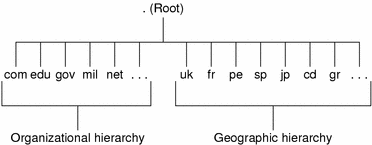
\includegraphics[scale=1]{image/hierarchy_dns}\label{hierarchy_dns}
\end{center}

Dzięki tej hierarchii systemu możemy powiedzieć o DNS, że charakteryzuje go bardzo dobra skalowalność oraz elastyczność. 

Jeśli chodzi o podział domen pierwszego poziomu ze względu na przynależność organizacyjną, to aktualny stan przedstawiony jest w tabeli poniżej.

\begin{table}[]
	\centering
	\caption{Podział domen najwyższego poziomu ze względu na działalność.}
	\label{my-label}
	\begin{tabular}{|r|p{10.5cm}|}
		\hline
		\textbf{TLD} & \textbf{Opis jednostki} \\
		\hline\hline
		com & Jednostki o działalności komercyjnej (ang. \textit{commercial institutions}) \\
		\hline
		edu & Jednostki edukacyjne (ang. \textit{educational institutions})\\
		\hline
		gov & Instytucje rządowe (ang. \textit{government institutions}) \\
		\hline
		mil & Grupy wojskowe (ang. \textit{military groupos}) \\
		\hline
		net & grupy związane z działaniem sieci (ang. \textit{network support centers}) \\
		\hline
		org & Organizacje nonprofit i inne (ang. \textit{nonprofit organizations}) \\
		\hline
		int & Organizacje międzynarodowe (ang. \textit{international organizations}) \\
		\hline 
	\end{tabular}
\end{table}

Przedstawiony podział nie jest stały. Autorzy zastrzegli, że w przysłości może być on rozszerzony o dodatkowe kategorie.

Podział ze względu na położenie geograficzne jest oczywiście bardziej naturalny i łatwy zarówno do wdrożenia jak i zrozumienia. Każdemu z państw przydzielono dwu bądź trzyliterowy identyfikator, który reprezentują domenę najwyższego poziomu odpowiadającą danemu państwu. Powołując się na informacje przedstawione na grafice \ref{hierarchy_dns} TLD o identyfikatorze \textit{uk} odpowiada domenom utożnasmianym z Wielką Brytnią, a \textit{fr} -- domenom francuskim.

Hierarchia systemu DNS wynika z faktu, że domenami internetowymi każdego poziomu może zarządzać inna organizacja. Odnosi się to zarówno do domeny \textit{root}, jak i domen nawyższego poziomu niezależnie od przynależności grupowej. W Polsce identyfikatorem TLD jest sufiks \textit{pl}, a jednostką odpowiedzialną za nią jest CERT Polska \cite{cert}. Jeśli użytkownik chciałby dołączyć ze swoją siecią do internetu powinien zgłosić do odpowiedniej organizacji taką chęć oraz dostarczyć wszystkich niezbędnych informacji które są wymagane przez zarządcę. 

Bardzo ważnym punktem jest wspomniana w poprzednim akapicie ,,chęć'' dołączenia do internetu. Jeśli uzytkownik czy organizacja chcą używać protokołu DNS jedynie do użytku wewnętrznego, to nie ma rystrykcyjnych ograniczeń co do używanych nazw. Jeśli natomiast oczekuje się wystawienia domen w taki sposób, aby były widoczne z zewnątrz, to należy odpowiednio:
\begin{enumerate}
	\item zarejestrować nazwę domeny,
	\item pozyskać adres IP.
\end{enumerate}

Bardzo trafne jest tu porównanie całego systemu Domain Name System do struktury plików w systemach operacyjnych z rodziny UNIX.  Nazwa domeny bezpośrednio określa jej miejsce w całej przestrzeni nazw, podobnie jak ścieżka bezwzględna pliku określa jego miejsce w całym systemie. Po rejestracji domeny, jest ona dołączana w odpowiednie miejsce w hierarchii. Przykład domeny \textit{google.com} razem z jej poddomenami i odpowiednimi miejscami w herarchii systemu przedstawiono na rysunku \ref{example_domain_tree}.

\begin{center}
	\begin{figure}
	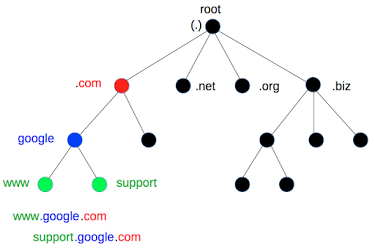
\includegraphics[scale=1]{image/domain_tree}\label{example_domain_tree}
	\caption{Położenie domeny w przestrzeni nazw. \cite{domain_tree_src}}
	\end{figure}
\end{center}

Serwer autorytatywny (ang. \textit{domain authority}) posiada odgórne przyzwolenie na zarządzanie nazwami swoich hostów (kto przyznaje(?)). Ze względu na drzewiastą strukturę systemu można oczekiwać, że kolejne domeny oraz ich serwery autorytatywne będą delegować odpowiedzialność za kolejne strefy do serwerów niższego poziomu. W ten sposób, powołując się na przykład przedstawiony na rysunku \ref{example_domain_tree} serwer autorytatywny com. zarządza nazwami w domenie com, natomiast zarządzanie nazwami w domenie google.com przekazuje do niższego szczeblem serwera przestrzeni nazw. W ten sposób serwer domeny google.com ma możliwość przypisywania nazw takim domenom jak zaprezentowane support.google.com.

\subsection{Domena DNS}
Domeną określa się dany podzbiór herarchii DNS. Są to wszystkie poddomeny podlegające tej samej domenie wyższego poziomu. Odnosząc się do wcześniej przywołanego porównania do systemu plików -- domena to odpowiednik folderu. Może zawierać kolejne domeny, może być określana zarówno na bardzo wysokim (domeny poziomu TLD) jak i bardzo szczegółowym(domeny 2-3 LD) poziomie abstrakcji. Jeśli chcielibyśmy reprezentować system DNS jako drzewo, to domeną DNS nazwiemy węzeł drzewa i wszystkie węzły które są jego potomkami. Pojęcie domeny i elementy które ono określa przedstawiono na rysunku \ref{domain_dns_example}.

\subsection{Strefa DNS}
Strefa DNS jest pojęciem, które określa zbiór domen za które odpowiedzialny jest konkretny serwer przestrzeni nazw. Jeśli wyobrazimy sobie hierarchię DNS jako drzewo, w którym węzłami są kolejne nazwy domen, to strefą DNS będzie zbiór węzłów tego drzewa. Zbiór węzłów wyznaczany jest na podstawie informacji o serwerze autorytatywnym odpowiedzialnym za daną domenę. Te węzły (domeny) których nazwami zarządza ten sam serwer znajdują się w jednej strefie DNS. Przykładowy podział systemu na konkretne strefy został zaprezentowany na rysunku \ref{dns_zone_example}.

\subsection{Strefa DNS a domena DNS}
System DNS danej domeny jest zrealizowany w oparciu o zbiór serwerów przestrzeni nazw (ang. \textit{nameserver}). Każdy z serwerów może być serwerem autorytatywnym dla pojedyńczej domeny, wielu domen bądź domen wraz z odpowiadającymi im poddomenami. Wycinek przestrzeni zarządzany przez określony serwer nazywany jest strefą DNS. 


\subsection{Kompletne nazwy domen}
Określeniem pełne, kompletne lub zupełne nazwy domen (ang \textit{Fully Qualified Domain Names (FQDNs)}) nazywane są te domeny, których nazwy zawierają domenę każdego poziomu, począwszy od lokalnej, aż po domenę główną, czyli root. Łatwo dostrzec analogię do wcześniej wspomnianego systemu pliku w systemach operacyjnych UNIX pomiędzy FQDN a bezpośrednią ścieżką do pliku. Różnicą jest tu jednak sposób odczytywania takiej ścieżki. W systemach DNS najbardziej ogólny węzeł znajduje się na skrajnie prawej pozycji a poruszając się w stronę lewą dochodzimy do kolejnych lokalnych domen. 

\subsection{Mapowanie nazw na adres IP}\label{mapping}
Mapowanie nazw domeny na jej adres IP jest możliwe dzięki plikom strefy DNS, które znajdują się na autorytatywnym serwerze przestrzeni nazw, tzw. \textit{zone files}. Jeden z typów tych plików przechowuje nazwy domen wraz z odpowiadającymi im adresami IP. Gdy klient chce dowiedzieć się pod jaki adres kierować swoje zapytanie, kieruje informacje do serwera autorytatywnego. On odpowiada za znalezienie i przedstawienie mapowania nazwy na adres IP, dokonując przeszukania plików strefy.

\subsection{Mapowanie odwrotne}\label{revmapping}
Baza danych DNS może także zawierać pliki, które umożliwiają mapowania odwrotne, tj. adresu IP na nazwę domeny/hosta. Mechanizm ten może być użyty przy próbie weryfikacji pochodzenia wiadomości. Chcąc wykluczyć próbę oszustwa ze strony prawdziwego nadawcy możemy posiłkować się właśnie odwrotnym mapowaniem. Możemy zweryfikować, czy adres IP mapowania odwrotnego zgadza się z adresem IP z którego nadano wiadomość. Mechanizm ten może być również wykorzystywany do autoryzacji operacji wykonywanych zdalnie. 

Odwrotne mapowanie wykorzystuje specjalną domenę \textit{in-addr.arpa}. Z założenia domena ta wykorzystuje adresy IP zamiast adresów domen.  Wspomniana domena jest częścią strefy DNS, która umożliwia takie właśnie odwzorowanie. Istotne jest, że adresy w domenie \textit{in-addr.arpa} są zapisywane w specyficzny dla siebie sposób -- od najniższego do najbardziej istotnego poziomu. Wynika z tego, że adresy IP w opisywanej domenie są w pewnym sensie zapisywane ,,od końca''. Powołując się na przykład, załóżmy, że maszyna ma przypisany adres 10.8.0.32. W plikach strefy dla domeny in-addr.arpa adres ten będzie zapisany jako 32.0.8.10.in-addr.arpa. oczywiście z kropką po członie \textit{in-addr.arpa}, która reprezentuje domenę \textit{root}.

\subsection{Wplisy plików strefy}
Tak jak wspomniano we wcześniejszych punktach \ref{mapping} oraz \ref{revmapping} działanie całego mechanizmu mapowana (czy to właściwego czy odwrotnego) może zachodzić dzięki serwerom autorytatywnym oraz przechowywanym przez nie plikom strefy DNS. 

Z racji, że system DNS dostarcza administratorom wielu funkcji poza standardowym mapowaniem adresów na IP, wpisy w bazach danych mogą być różnych typów. Najpopularniejsze typy to oczywiście te, z którymi można zetknąć się na codzień, na przykład wpis typu \textit{A} -- tłumaczący nazwę hosta na adres IP w wersji 4, \textit{AAAA} -- mapujący nazwę hosta na adres IP w wersji 6, rekordy \textit{CNAME} służące do aliasów, czy MX -- specyfikujące serwer wymiany wiadomości elektronicznych dla danej domeny. Oprócz wspomnianych podstawowych typów twórcy standardu dla systemu DNS wprowadzili także mniej znane typy. Opis zbioru najbardziej istotnych wpisów określonych w dokumencie RFC 1035 \cite{RFC1035} wraz z ich przeznaczeniem umieszczono w tabeli \ref{typyRekordowDns}.

\begin{table}[]
	\centering
	\caption{Rodzaje rekordów w bazach danych serwerów przestrzeni nazw. Opis na podstawie \cite{}}
	\label{typyRekordowDns}
	\begin{tabular}{|r|p{3cm}|p{8cm}|}
		\hline
			\textbf{Rekord} & 
			\textbf{Pełna nazwa} & 
			\textbf{Pełniona funkcja(opis zawartości)} \\
		\hline\hline
			A & 
			Wpis mapowania adresów(ang. \textit{Address mapping record}) & 
			Określa adres IP wersji 4 dla danego hosta. Służą do konwersji nazwy domen do opowiednich adresów IP.\\
		\hline
			CNAME & 
			Nazwa kanoniczna (ang. \textit{Canonical Name)} & 
			\\
		\hline
			MX & 
			Wymiana wiadomości elektronicznych (ang. \textit{Mail exchange)} & 
			\\
		\hline
			NS & 
			Serwer nazw (ang. \textit{Name server)} & 
			\\		
		\hline
			SOA & 
			Początek (ang. \textit{Start of Authority)} & 
			\\
		\hline
			TXT & 
			Tekst & 
		\\
		\hline
		
	\end{tabular}
\end{table}

Oczywiście na przestrzeni lat protokół rozszerzano o kolejne funkcje. Jednym z istotnych wydarzeń było zaproponowanie zmian spisanych w dokumencie RFC 4034 \cite{}. Opisano tam rozszerzenia protokołu DNS, które podnoszą jego bezpieczeństwo. W tabeli \ref{typyRekordowDnsExt} przedstawiono najważniejsze z punktu widzenia niniejszej pracy typy rekordów, które zostały wprowadzone w kolejnych dokumentach RFC, których dokładne numery zostały wspomniane przy konkretnych wpisach w tabeli. 

\begin{table}[]
	\centering
	\caption{Rodzaje rekordów w bazach danych serwerów przestrzeni nazw określonych w rozszerzeniach dokumentu RFC 1035 \cite{}.}
	\label{typyRekordowDnsExt}
	\begin{tabular}{|r|p{3cm}|p{8cm}|}
		\hline
		\textbf{Rekord} & 
		\textbf{Pełna nazwa} & 
		\textbf{Pełniona funkcja(opis zawartości)} \\
		\hline\hline
			AAAA & 
			Wpis mapowania adresów IPv6 & 
			Określa adres IP wersji 6 dla danego hosta. Zasada działania jest taka jak w przypadku rekordu A z jedyną różnicą w wersji adresu IP. \\
		\hline
	\end{tabular}
\end{table}

\subsection{TLD ARPA}
Specyficzną domeną najwyższego rzędu jest domena \textit{ARPA}.

\subsection{Domena 2LD e164}

\subsection{Domena 2LD in-addr}

\section{Transfer stref DNS}

\subsection{Transfer AXFR}

\subsection{Transfer IXFR}

\section{Podpisy TSIG}\label{TSIG}
Istotnym typem rekordu jest również typ 250. -- rekord TSIG(ang. \textit{Secret Key Transaction Authentication for DNS/Transaction Signature}) zdefiniowany w dokumencie RFC 2845\cite{RFC2845}. Używany jest przede wszystkim w protokole DNS aby zapewnić, że informacja przesyłana pomiędzy obiema komunikującymi się stronami faktycznie pochodzi od nadawcy oraz że nie była modyfikowana w trakcie komunikacji. System uzywany jest przede wszystkim do dynamicznych aktualizacji baz DNS oraz do transferów stref pomiędzy serwerem głównym a podrzędnym. Aby komunikacja była kryptograficznie bezpieczna, w protokole wykorzystywane są klucze tajne oraz bezkolizyjne funkcje skrótu.

\subsection{Opis działania TSIG}
Rekord TSIG pozwala na wykorzystywanie mechanizmów znanych z protokołu DNSSEC\cite{nask-tsig} w protokole DNS zaproponowanych w RFC 1035\cite{RFC1035}. Praktyka taka została zaproponowana z powodu częstych problemów z używaniem protokołu DNSSEC\cite{RFC4033, RFC4035}. Wprowadzenie korzystania z rekordów TSIG pozwala między innymi na:
\begin{enumerate}
	\item kontrolowanie aktualizacji stref DNS,
	\item zabezpieczenie transferu strefy DNS,
	\item zabezpieczenie komunikacji pomiędzy aktorami (na przykład pomiędzy serwerami przestrzeni nazw).
\end{enumerate}

Zgodnie z nazwą, rekord TSIG jest w głównej mierze kontenerem mającym za zadanie przechowywanie podpisu danej wiadomości DNS. Gdy zostanie wykorzystany jest porzucany zatem nie ma powodu, dla którego rekordy tego typu powinny być przechowywane przechowywane. TSIG znajduje się w części dodatkowej APDU DNS. Po odebraniu pakietu zawierającego TSIG, odpowiedni rekord z sekcji dodatkowej zostaje usunięty i zapisany w oddzielnym miejscu w pamięci. Nagłówek wiadomości jest odpowiednio modyfikowany, tak aby pola dłogości jak i liczby odpowiedzi od serwerów były zgodne z faktycznym stanem po dokonanej modyfikacji. Następnie liczony jest skrót wiadomości z wstępnie przeprocesowanego pakietu i porównywany z podpisem zapisanym uprzednio w innym miejscu w pamięci. W sytuacji, gdy wartość obliczona przez funkcję skrótu jest różna od wartości odebranej w rekordzie TSIG razem z całą odpowiedzią DNS pakiet taki należy odrzucić oraz powiadomić o tym fakcie nadawcę wiadomości. Rekord TSIG niesie także informacje o dwóch czasach: pierwszy -- kiedy utworzono skrót oraz drugi -- jak długo skrót zachowuje swoją ważność. Weryfikacja odebranego pakietu obejmuje nie tylko wartość funkcji skrótu ale także opisany czas. Jeśli czas odebrania wiadomości nie zawiera się w okresie jej ważności odsyłany jest komunikat o błędzie. Dodanie czasu utworzenia pakietu było konieczne, aby zabezpieczyć się przed atakami odtworzeniowymi, gdzie atakujący wykorzystuje podsłuchany pakiet ponownie. Wykorzystywanie stempli czasowych wymaga użycia odpowiedniego zegara. Nie jest to problem jeśli maszyna jest podłączona do internetu, ponieważ może być wykrozystany wtedy protokół NTP (ang. \textit{Network Time Protocol})\cite{RFC5905}.

Generowanie podpisanej odpowiedzi może mieć miejsce tylko po odebraniu podpisanego zapytania od klienta. Serwer nie może wysłać odpowiedzi zawierającej rekord TSIG jeśli otrzymał niepodpisane zapytanie. Generacja skrótu znajdującego się w odpowiedzi składa się zarówno ze skrótu który przysłał klient jak i zawartości rekordu TSIG\cite{nask-tsig}.

Użycie mechanizmu podpisywania wiadomości eliminuje może eliminować problem nieuprawnionego transferu danych. Z pewnością wyklucza użycie algorytmu wykorzystywanego w niniejszej pracy magisterskiej, gdyż łamanie nawet prostych kluczy wielokrotnie zwiększa czas procesowania pojedyńczej domeny\cite{nask-tsig}. Oczywiście zabezpieczenie kluczy używanych do podpisywania wiadomości a także ich długość i jakoś są bardzo ważne w kwestii poziomu bezpieczeństwa protokołu. Zaleca się, aby długość generowanego skrótu była mniejsza bądź równa długości klucza użytego do podpisania wiadomości.

\subsection{Wady TSIG}\label{wady-tsig}
Problemem związanym z wykorzystaniem rekordów TSIG jest przede wszystkim dystrybucja kluczy. Ponadto w systemie DNS rzadko zdarza się, że tylko jeden klient będzie korzystał z interfejsu serwera, więc każdy z klientów powinien posiadać swój klucz, co ponownie prowadzi do problemu ich dystrybucji, przechowywania i zarządzania\cite{nask-tsig}. 

Inną istotną wadą protokołu jest rodzaj zaproonowanej funkcji skrótu HMAC-MD5. Algorytm ten nie jest uważany w dzisiejszych czasach za bezpieczny. Ataki na HMAC-MD5 zaprezentowano między innymi w pracach \cite{hmac-md5-attack, hmac-md5-cryptoanalisys}. 

Kolejnym problemem a raczej niedoskonałością zaproponowanego rozwiązania jest zupełnie płaska stuktura. Oznacza to tyle, że na poziomie podpisanych wiadomości przy użyciu TSIG nie mamy dostępnych żadnych poziomów herarchii. Jeśli wiadomość spełnia wymogi formalne, czyli ma poprawne stemple czasowe oraz dobrze wyznaczoną wartość funkcji skrótu to traktowana jest dokładnie tak samo jak inna poprawna wiadomość, bez rozróżnienia z jakiego źródła pochodzi. Gdy mówimy o protokole DNS, gdzie jednym z kluczowych elementów jest hierarchiczna struktura musimy liczyć się z faktem, że mechanizm TSIG może być nieodpowiedni.

\section{Inne metody podpisywania wiadomości}
Oprócz przedstawionego w podpunkcie \ref{TSIG} mechanimzu TSIG postało kilka innych propozycji podpisywania wiadomości w protokole DNS. Propozycje te opracowaywane były przede wszystkim dlatego, że TSIG charakteryzuje się pewnymi uciążliwymi wadami opisanymi w podpunkcie \ref{wady-tsig} -- nie rozwiązuje problemu dystrybucji kluczy, nie uwzględnia poziomów w hierarchii systemu DNS czy wykorzystuje przestarzałą funkcję skrótu HMAC-MD5.

Niektóre propozycje skupiały się jedynie na zabezpieczaniu dynamicznych aktualizacji wpisów rekordów DNS \cite{RFC2137} a inne rozwiązywały tylko problemy bezpiecznej, skutecznej i automatycznej dystrybucji kluczy pomiędzy stronami protokołu -- serwerem oraz resolwerem\cite{RFC2930}. Wymiana kluczy opisana w dokumencie \cite{RFC2930} miałaby odbywać się dzięki nowemu typowi rekordu DNS -- TKEY (ang. \textit{transaction key}).

Powstawały także rozwiązania rozszerzające TSIG jak na przykład algorytm zaproponowany w RFC3645\cite{RFC3645}. Wykorzystuje się w nim GSS\cite{RFC2743}(ang. \textit{Generic Security Service}) aby zapewnić bezpieczną u automatyczną dystrybucję kluczy do klientów protokołu TSIG. Bardziej generyczna metoda wymiany kluczy była opisana w RFC2930\cite{RFC2930}, gdzie wykorzystanie GSS-API było tylko jedną z możliwości rozwiązania postawionego problemu.

Innym kierunkiem rozwoju protokołu TSIG jest wykorzystywanie innych algorytmów implementujących funkcje skrótu. Spowodowane jest to faktem, że RFC2845\cite{RFC2845} definiuje wykorzystanie jedynie funkcji HMAC-MD5. Jedną z takich prób opisano w dokumencie RFC4635\cite{RFC4635} gdzie zaproponowano zastąpienie przestarzałej funkcji MD5 funkcjami z rodziny SHA. Opisano odpowiednio użycie SHA1\cite{RFC3174} lub algorytmów zaproponowane w projekcie FIPS PUB 180-2, znane później jako SHA-2\cite{RFC4634}.

\chapter{Przegląd dostępnych narzędzi}
Społeczność internetu oferuje bardzo szeroką gamę narzędzi umożliwiających pozyskiwanie informacji na podstawie protokołu DNS. Bardzo użytecznym i przydatnym narzędziem jest w tym przypadku program dig. Wspomniany program ma jednak znaczącą wadę -- jest wydajny jedynie przy niewielkiej liczbie odpytywanych domen. Dodatkową niedogodnością jest, wbrew pozorom, fakt, że program wchodzi w skład pakietu Open Source bind. Ten, jak każde oprogramowanie na wolnej licencji, cierpi na szereg niedogodności z tym związanych. Najbardziej prozaicznym problemem jest fakt, że oprogramowanie jest tworzone przez wiele osób, więc bardzo trudno zastosować jeden standard kodowania, gdyż każda z osób ma swój preferowany. Poza tym, dużą wadą jest trudność wprowadzania zmian w tego typu oprogramowaniu, wynikająca zarówno z punktu poprzedniego jak i ze złożoności programu, którą cechuje się dig w tym momencie.

Istnieją także inne pakiety implementujące w dość wydajny sposób klienta systemu DNS jak np. pjlib \cite{pjlib}. Również w tym przypadku można borykać się z problemami wynikającymi z założeń przyjętych przez twórców tego oprogramowania. Koknkretyzując to stwierdzenie - wspomniana biblioteka z założenia miała być wykorzystywana do protokołu SIP, a więc implementacja klienta DNS weszła w jej skład tylko i wyłączenie dlatego, że twórcy jej potrzebowali jako narzędzia do zrealizowania innych celów. Implikuje to fakt, że pobieranie wiadomości jest niekompletne na płaszczyźnie typów wiadomości. Jednym z nich jest typ nr 252, czyli AXFR, który jest jednym z kluczowych elementów rekonsesansu na podstawie protokołu DNS.
\chapter{Powiązane prace}
Pomimo faktu, że problem ,,wycieku'' danych z serwerów DNS jest dość powszechnie poruszany zarówno w różnego rodzaju publikacjach\cite{} jak i na blogach dotyczących testowania infrastruktury pod kątem bezpieczeństwa\cite{}, to nie udało dotrzeć się do żadnych globalnych badań na temat bezpieczeństwa transferu strefy DNS. To właśnie skala badania przeprowadzonego w ramach niniejszej pracy magisterskiej jest główną różnicą w stosunku do badań już przeprowadzonych. Ponadto, bardzo ważnym założeniem przedstawionym w tej pracy jest chęć nakreślenia skali zjawiska nieuprawnionego transferu danych DNS. Określenie jak duży jest to problem jest konieczne do odpowiedniego wydania ewentualnych zaleceń oraz przyporządkowania priorytetu bądź rangi tej podatności. W poniższym rozdziale przedstawiono powiązane prace oraz ich różnice w stosunku do opisywanych badań.

\section{DNS Response Policy Zone}


\section{Internet-Wide Scan Data Repository}
\textit{Internet-Wide Scan Data Repository} jest to publiczne archiwum danych dostępne głównie pod adresem scans.io\cite{scansio}. Gromadzone są tam dane badawcze zebrane podczas aktywnych skanów przeprowadzonych w internecie. Repozytorium prowadzone jest przez badaczy z Uniwersytetu z Michigan\cite{teamcensys}. Cel pobierania danych nie jest wyraźnie określony przez naukowców, to co zostanie z nich wywnioskowane pozostawia się osobom trzecim. Z punktu widzenia niniejszej pracy, \textit{Internet-Wide Scan Data Repository} może posłużyć jako punkt odniesienia na przestrzeni skanowania AXFR. Na stronie możemy znaleźć wyniki aktywnego skanowania domen z listy Alexa Top 1 Milion\cite{alexa} pod kątem podatności na nieuprawniony transfer strefy DNS.

Jednym z udogodnień ze strony pracowników Uniwersytetu z Michigan jest udostępnienie wygodnego interfejsu dla ludzi. Zarządcy opisywanego repozytorium danych udostępniają również aplikację, wyszukiwarkę informacji na temat domen przeskanowanych pod różnym kątem w ich badaniach. Cały projekt nosi tę samą nazwę co zespół -- Censys\cite{censys} i pozwala wyszukiwać informacje zarówno po adresach URL/IP jak i po zawartości odpowiedzi uzyskanych ze skanów.

Różnicą która jest pomiędzy pracami opisanymi w tym punkcie a niniejszą pracą magisterką jest oczywiście zasięg prowadzonych badań. Ograniczenie się jedynie do miliona najpopularniejszych domen, tak jak to zrobił zespół Censys\cite{censys} jest bardoz dużym uproszczeniem. Ponadto, naturalne jest, że najpopularniejsze strony będą przykłądały dużo uwagi do odpowiedniego zabezpieczenia swoich zasobów, dlatego można się spodziewać, że wyników takiego skanowania będzie mniej niż na równej ilościowo, losowo wybranej próbie. 

\section{DNS as a service}
DNS as service to pojęcie wykorzystywane do opisywania usług świadczonych w obrębie protokołu DNS. Dosłownym tłumaczeniem tego terminu jest \textit{DNS jako usługa}. W rozumieniu protokołu DNS jest to ograniczone do wystawienia interfejsów klientowi, tak, aby mógł on dodać interesujące go rekordy. 

\textit{DNS as a service} spotykane jest najczęściej w kontekście unikania ataków DDoS jednak mimo to można przyjrzeć się temu zjawisku również przy okazji analizy bezpieczeństwa transferu strefy DNS. Określenie \textit{Distributed Denial of Service} jest w tym przypadku swego rodzaju chwytem marketingowym, ponieważ najbardziej efektywnie działa na wyobraźnię klientów. Niemniej jednak, bezpieczeństwo systemów DNS to nie tylko unikanie ataków DDoS. 

Tym, co faktycznie sprzedają firmy oferujące usługi \textit{DNS as a service} jest przede wszystkim infrastruktura, ale także pewnego rodzaju bezpieczeństwo informacji oraz pewność dostępności systemu DNS. Dobrym przykładem jest w tym przypadku oferta firmy Nexusguard\cite{nexusguard}. Oferuje ona obsługę oraz zabezpieczenie systemu DNS swojego klinta. Wprowadzenie danych na temat strefy DNS klienta może odbywać się na dwa sposoby:
\begin{enumerate}
	\item poprzez panel klienta,
	\item poprzez transfer strefy DNS z serwera klienta.
\end{enumerate}
W kontekście tej pracy magisterskiej pierwszy przypadek nie jest nadzwyczaj interesujący. Klient uzupełnia dane o rekordach DNS swojej domeny czy też strefy i cała odpowiedzialność za rozwiązywanie kolejnych zapytań jest przeniesiona na maszyny działające pod nadzorem firmy oferującej usługę. Dużo bardziej interesującym przypadkiem jest wymieniony jako drugi transfer strefy z serwera klienta. Wydzielona część infrastruktury firmy jest wtedy traktowana jako zapasowy serwer DNS(\textit{ang. slave}) podczas gdy serwerem podstawowym (\textit{ang. primary}) jest maszyna klienta. Transfer strefy DNS jest dużo bardziej bezpieczny. Wynika to z wymagań narzuconych przez organizację, mowa między innymi o mechanizmie TSIG (\textit{ang. Transaction Signature})  opisanym w rozdziale \ref{} oraz wykorzystaniu połączenia szyfrowanego opartego na SSL pomiędzy serwerem podstawowym a podrzędnym. Jeśli chodzi o bezpieczeństwo dostępu do rekordów DNS poprzez panel kliencki, to możliwe jest wykorzystanie dwuetapowej weryfikacji użytkownika.

Warto dodać, że \textit{DNS as a service} jest również w ofercie kilku innych, na przykład Akamai\cite{akamai}, CloudFlare\cite{cloudflare} czy Imperva\cite{incapsula}. Obecność usług takich jak DNS as service sugeruje, że jest to bardzo istotne, aby odpowiednio zabezpieczać nie tylko główne maszyny i usługi w swojej sieci ale i niemal każdy element, który działa w naszym systemie. Dodatkowo sugeruje to, że często administratorzy czy klienci wolą przenieść odpowiedzialność za utrzymywanie takiego systemu na firmę trzecią w zamian za odpowiednie ich wynagrodzenie.

\section{DNS Enumeration}
Rozszerzenie DNSSEC \textit{DNS Security Extentions} zostało zaprezentowane w roku 1997\cite{RFC2065} jako odpowiedź na poważne luki w bezpieczeństwie systemów DNS opisane w dokumencie \cite{DNSsecurityProblem}. W dużym uproszczeniu rozszerzenie to pozwala na zweryfikowanie, czy odpowiedź na zapytanie wysłane do serwera pochodzi na pewno od niego a nie od atakującego system. Wyspecyfikowanie standardu DNSSEC było problematyczne, a organizacje pracujące nad nim wielokrotnie go zmieniały. Podyktowane to było różnego rodzaju ograniczeniami technicznymi. Jednym z takich ograniczeń technicznych jest zjawisko \textit{DNS Enumeration} (lub \textit{Zone Enumeration}). Jest to podatność w sieci polegająca na wylistowaniu wszystkich urządzeń, które do tej sieci należą. W standardzie DNSSEC umożliwiono \textit{zone enumeration}, którego wynikiem były nawet urządzenia sieciowe (na przykład rutery) znajdujące się w danej strefie. Zjawisko nie jest luką krytyczną, jednak może prowadzić do bardziej złożonych ataków. 

Problem listowania strefy DNS wynika z różnego traktowania odpowiedzi pozytywnej oraz negatywnej od serwera. Odpowiedź pozytywna jest wysyłana w przypadku, gdy dana domena istnieje oraz przypisano jej adres IP. Przykładowo:
\begin{enumerate}
	\item Klient: Jaki jest adres domeny www.przyklad.pl?
	\item Serwer: Domena www.przyklad.pl ma adres 1.2.3.4.
\end{enumerate} 
Jeśli chodzi o odpowiedź negatywną, to przykład podano poniżej:
\begin{enumerate}
	\item Klient: Jaki jest adres dla domeny nieistnieje.przyklad.pl?
	\item Serwer: Domena nieistnieje.przykład.pl nie istnieje.
\end{enumerate}

Oba przytoczone powyżej przypadki są w pewnym stopniu inaczej traktowane w protokole DNSSEC. Dla przykładu, gdy odpowiedzią jest adres IP istniejącej domeny, serwer autorytatywny przechowuje określony, skońcozny zbiór podpisanych rekordów. Podpisy są tworzone przy użyciu klucza prywatnego danej domeny. Istotny jest fakt, że podpisy rekordów nie są obliczane w czasie rzeczywistym, a jedynie przechowywane razem z innymi rekordami w bazie danych DNS. Zaletą takiego rozwiązania jest oczywiście redukcja obliczeń wykonywanych przez serwer autorytatywny a poza tym, tylko jeden z serwerów musi być w posiadaniu klucza prywatnego, więc dystrybucja klucza jest w dużym stopniu uproszczona. Dodatkowo w przedstawionym wcześniej modelu nie ma potrzeby, aby weryfikować tożsamość każdego z serwerów w systemie DNS, co ponownie upraszcza komunikację, zmniejsza obciążenie w sieci oraz ilość informacji.

Problem listowania strefy DNS pojawia się wraz z charakterystyczną, negatywną odpowiedzią (w specyfikacji określaną jako NXDOMAIN). Nie jest możliwe, aby odpowiadać na pytanie o niepoprawną domenę wcześniej przygotowaną wiadomością z obliczonym skrótem, ponieważ może to prowadzić do skutecznego ataku odtworzeniowego (ang. \textit{reply attack}). Nie jest możliwe obliczenie wsyzstkich skrótów, dla każdej z poddomen, bo takich przypadków jest zbyt wiele. Ciężko także zrezygnować z niewątpliwej zalety przytoczonej w poprzednim akapicie -- braku konieczności obliczania skrótów w czasie rzeczywistym. Pomysłodawcy rozwiązania opisanego w RFC4034\cite{RFC4034} zaproponowali algorytm, dzięki któremu możliwe będzie utrzymanie substytutu podpisanej wiadomości NXDOMAIN. Cały system zachowuje również zalety przedstawione w poprzednim akapicie. Rozwiązanie zakłada, że rekordy w strefie są uporządkowane, każda para rekordów jest podpisana i tworzy rekord NSEC a każdy rekord podpisany kluczem prywatnym. Jeśli serwer odbierze zapytanie o domenę, która nie istnieje, odpowiada rekordem NSEC pary domen które w uporządkowanej liście znajdują się odpowiednio przed i po odpytywanej domenie oraz związane z nimi podpisy. Rozwiązanie zapewnia, że tylko serwer autorytatywny powinien być obdarzony zaufaniem oraz umożliwia wstępną generację podpisów. Niestety wprowadza dodatkowo efekt uboczny, w postaci umożliwenia \textit{zone enumeration}, czyli wylistowania strefy.

Zagadnienie listowania stref DNS samo w sobie często było podmiotem dyskusji. Początkowo wydano dokument, że nie jest to błędem, że umożliwia się wypisanie bazy danych DNS\cite{RFC4033}. Później jednak wypracowany został kompromis\cite{RFC5155}, że w pewnych przypadkach znajomość wszystkich domen może powodować dodatkowe niebezpieczeństwa. Przykłady, które przytoczono w RFC5155\cite{RFC5155} to na przykład dobre źródło danych wejściowych, które mogą posłużyć jako prawdopodobne adresy mailowe w kampaniach spamowych bądź jako informacje o infrastrukturze wykorzystywane podczas rekonesansu DNS. Ponadto podatność nazywana \texit{zone enumeration} może afektować na organizacje zajmujące się rejestrami DNS. Często są one zobowiązane do nieujawniania danych przechowywanych w soich rejestrach. Rekord NSEC umożliwia przeprowadzenie \texit{DNS enumeration} na strefach tych organizacji a następnie wykonanie zapytań whois\cite{RFC3912} w celu pozyskania informacji o osobie rejestrującej domenę. 
\chapter{Implementacja}
Przeanalizowanie problemu postawionego w niniejszej pracy magisterskiej wymagało implementacji własnych narzędzi. Jak wcześniej
wspomniano, programy dostępne w sieci są bardzo dobre (dig \cite{dig}, axfr-tool \cite{python_axfr_test}, robotex \cite{robotex})
jednak nie zapewniają oczekiwanej wydajności. Wynika to z faktu, że są one nastawione głównie na analizę konkretnego przypadku.
Narzędzia są używane głównie przez pentesterów, których typowym zadaniem jest przetestowanie pod kątem bezpieczeństwa na przykład pewnej
aplikacji, gdzie liczba serwerów DNS jak i testowanych domen jest mocno ograniczona. Proces ten sam w sobie jest niezwykle złożony
i często wymaga nawet tygodni pracy, dlatego czas w jakim wykonywał się będzie program sprawdzający podatności DNS nie jest aż tak
istotny. Oczywiście mówimy o różnicy w czasie w granicach do kilku minut. W podejściu prezentowanym w tej pracy założono, że
przeanalizuje się możliwie jak najwięcej domen dostępnych w sieci internet. Dlatego też różnica procesowania jednej pary
domena -- adres IP serwera autorytatywnego już nawet na poziomie kilku sekund pozwala zaobserwować bardzo duży skok wydajności.

Dojście do rozwiązania optymalnego nie było trywialne. Początkowe rozwiązania opierały się na próbach rozszerzenia dostępnych
narzędzi o managera
zarządzającego procesami, w których uruchamiane były zewnętrzne narzędzia -- głównie dig. Rozwiązanie takie miało szereg zalet,
na przykład było bardzo skalowalne i łatwe do zrealizowania. Niestety okazało się, że menedżer zarządzający procesami wymaga
zbyt dużej ilości zasobów, a głównie pamięci RAM, dlatego wymuszone zostało zrezygnowanie z tego podejścia.

\section{Przegląd dostępnych narzędzi}
Społeczność internetu oferuje bardzo szeroką gamę narzędzi umożliwiających pozyskiwanie informacji na podstawie protokołu DNS.
Bardzo użytecznym i przydatnym narzędziem jest w tym przypadku program dig. Wspomniany program ma jednak znaczącą wadę -- jest
wydajny jedynie przy niewielkiej liczbie odpytywanych domen. Dodatkową niedogodnością jest, wbrew pozorom, fakt, że program
wchodzi w skład pakietu Open Source bind. Ten, jak każde oprogramowanie na wolnej licencji, cierpi na szereg niedogodności z
tym związanych. Najbardziej prozaicznym problemem jest fakt, że oprogramowanie jest tworzone przez wiele osób, więc bardzo
trudno zastosować jeden standard kodowania, gdyż każda z osób ma swój preferowany. Poza tym, dużą wadą jest trudność wprowadzania
zmian w tego typu oprogramowaniu, wynikająca zarówno z punktu poprzedniego jak i ze złożoności programu, którą cechuje się dig
w tym momencie.

Istnieją także inne pakiety implementujące w dość wydajny sposób klienta systemu DNS jak np. pjlib \cite{pjlib}. Również w tym
przypadku można borykać się z problemami wynikającymi z założeń przyjętych przez twórców tego oprogramowania. Konkretyzując to
stwierdzenie - wspomniana biblioteka z założenia miała być wykorzystywana do protokołu SIP, a więc implementacja klienta DNS
weszła w jej skład tylko i wyłączenie dlatego, że twórcy jej potrzebowali jako narzędzia do zrealizowania innych celów.
Implikuje to fakt, że pobieranie wiadomości jest niekompletne na płaszczyźnie typów wiadomości. Jednym z nich jest typ nr 252,
czyli AXFR, który jest jednym z kluczowych elementów rekonesansu na podstawie protokołu DNS.

\section{Zaimplementowane narzędzia}
Przeprowadzenie globalnego skanu niosło za sobą szereg konsekwencji. Zakładając, że średnio należy przeznaczyć na skanowanie
jednej pary (domena, adres IP) około 3 sekund okazało się, że przeprocesowanie całego zbioru danych wejściowych (ok. 5 miliardów
par) zajęłoby odpowiednio:
$$3(s) * 5 * 10^{9} = 25 * 10^{8}(min) = \frac{25}{60} * 10^{8}(h) = 41.67 * 10^{6} (dni)\label{obliczenia}$$
Opierając się na opisanym wyżej rozumowaniu, podjęto decyzję, że należy procesować pary (domena, adres IP) równolegle.
Podjętych zostało kilka prób implementacji odpowiedniego narzędzia umożliwiającego przeprowadzenie badań w zadowalającym czasie:
\begin{itemize}
	\item narzędzie oparte na programie dig skryptach powłoki bash,
	\item menadżer procesów programu dig oparty na skryptach języka Python,
	\item skaner AXFR (C-AXFR) wspomagany skryptami powłoki bash.
\end{itemize}
Szczegółowo zostaną one opisane w kolejnych punktach tego rozdziału.

\subsection{Program dig zarządzany skryptami powłoki}
\label{dig_sh}
Pierwszym rozwiązaniem, które powstało w ramach pracy nad opisywanym problemem był skaner AXFR oparty na programie
dig \cite{isc}. Program skupia się wokół protokołu DNS i umożliwia wykonywanie zapytań różnych typów \cite{Liu:2006:DB:1197828}.
Ponadto, jest prosty w obsłudze, daje duże możliwości jeśli chodzi o budowanie zapytań DNS oraz bardzo często dostępny jest
domyślnie w wielu dystrybucjach systemów operacyjnych Linux.

Odpowiedzi uzyskane dzięki programowi miały być zapisywane do plików tekstowych. Każda, potencjalnie uzyskana odpowiedź miała
być zapisywana do oddzielnego pliku tekstowego, aby wykluczyć równoczesne użycie tego samego zasobu przez wiele procesów.
Rozwiązanie tego typu działa oraz z powodzeniem przeskanowano kilka tysięcy domen, jednak okazało się zbyt wolne do zastosowania
na szerszą skalę a także występowały kłopoty z zapotrzebowaniem na zasoby (mowa tu głównie o pamięci operacyjnej). Bliźniacze
podejście zostało zastosowane w opisywanym wcześniej projekcie skanowania domen z listy \textit{Alexa 1 Milion} \cite{scans.io}.

\subsection{Menedżer procesów zarządzany skryptami języka Python}
Kolejną próbą rozwiązania problemu ogromnej liczby danych do przeskanowania była implementacja skanera w języku skryptowym Python.
Próba ta podyktowana była kilkoma istotnymi aspektami. Pierwszym z nich jest implementacja tak zwanych ,,programowych'' wątków w
standardowej bibliotece tego języka. Umożliwiło to implementację mechanizmu, który pozwolił sprawdzić, czy maszyna dysponuje
takimi zasobami, które pozwolą na uruchomienie kolejnego wątku skanującego. Dodatkowym atutem jest tu także możliwość wywoływania
poleceń powłoki systemu Linux ze skryptu języka Python, a więc możliwe było wykorzystanie istniejącej już implementacji programu
dig \cite{isc}.

Niestety podobnie jak we wcześniej opisywanym przypadku, problemem okazały się ograniczenia czasowe spowodowane niewystarczającą
ilością zasobów. Program został przetestowany podczas kilkudniowego skanowania i zdołano odpowiednio:
\begin{itemize}
	\item przeanalizować kilka milionów par (domena, adres IP),
	\item pozyskać dane do wstępnej analizy podatności w skali globalnej,
	\item dwukrotnie zawiesić maszynę, na której wykonywano badania.
\end{itemize}

Pomimo, że implementacja w języku Python nie okazała się na tyle wydajna aby wykorzystać ją w badaniach przeprowadzonych w
ramach tej pracy magisterskiej, jest to dobrze narzędzie dla pasjonatów bezpieczeństwa sieciowego, którzy chcą skanować wiele
serwerów. Podejście takie zaprezentowane jest w kilku projektach, które można znaleźć w serwisie github na przykład
Python-AXFR-test \cite{python_axfr_test} lub skanowanie domen z Alexy wraz ze wstępną analizą wyników \cite{asg-axfr}. Liczba osób,
które śledzą wymienione wyżej projekty znajduje się w przedziale kilkudziesięciu osób. (?? Sporne) Również na tej podstawie możemy zakładać,
że temat bezpieczeństwa transferów strefy cieszy się zainteresowaniem wśród pasjonatów bezpieczeństwa sieci. (??)

Można przypuszczać, że oba projekty zrealizowane w języku Python \cite{python_axfr_test, asg-axfr} oferują podobną wydajność do
rozwiązania zaimplementowanego podczas realizacji pracy magisterskiej, jednak nie były prowadzone pomiary pod tym kątem. Brak
bezpośredniego porównania wynika z faktu, że prace Stephena Haywooda \cite{asg-axfr} były prowadzone niemal równolegle z realizacją
niniejszej pracy magisterskiej, zaś skrypt Python-AXFR-test \cite{python_axfr_test} jest jednowątkowy i nastawiony głównie na test
pojedynczych serwerów, więc jego wykorzystanie wymagałoby implementacji bardzo podobnego mechanizmu, który opisywany był na
początku tego rozdziału.

\subsection{Skaner C-AXFR}
Ostatecznie zdecydowano się na napisanie własnego narzędzia umożliwiającego transfer strefy DNS. Wybór padł na język
programowania C \cite{Kernighan:1988:CPL:576122} w wersji standardu C11 \cite{ISO9899}. Oczywiście aplikacje pisane w języku
C nie należą do rozwiązań prostych, jednak są bardzo dobrym kompromisem pomiędzy wysokim poziomem abstrakcji modeli programistycznych
i łatwością dostępu do interfejsów sieciowych. Ponadto język C charakteryzuje się dość dobrą szybkością działania, ze względu na
kompilację kodów źródłowych do kodu binarnego. Kryterium szybkości działania było jednym z kluczowych przy implementacji, co
pokazały poprzednie próby implementacji.

Rolę danych wejściowych programu mogą pełnić odpowiednio:
\begin{enumerate}
	\item plik tekstowy w formacie \textit{adres\_domeny}|\textit{IP\_serwera\_autorytatywnego},
	\item para parametrów wejściowych podanych w odpowiedniej kolejności - \textit{adres\_domeny IP\_serwera\_autorytatywnego}.
\end{enumerate}
Zdecydowano się na takie rozróżnienie z prostego powodu. Najistotniejszą kwestią prezentowanego rozwiązania było
zachowanie podobieństwa do programu dig, który jest wykorzystywany przez wiele osób. Dodatkowo, dużo łatwiej można testować
logikę programu na małych
porcjach danych i opcja numer 2. została w pewnym sensie funkcją debugową. Jako wspomniane dane testowe najczęściej wykorzystywana
była domena \textit{zonetransfer.me} \cite{zonetransfer}, której autor specjalnie umożliwia transfer strefy, aby uzmysłowić innym
ludziom zagrożenie wynikające z niepowołanego korzystania.

Logika programu jest bardzo prosta. Początkowo budowana jest jednostka APDU protokołu DNS z odpowiednimi danymi, a w szczególności
z poprawnie ustawioną flagą \textit{qtype} odpowiedzialną za identyfikację rodzaju zapytania DNS. Co ważne, mechanizm AXFR wymaga
używania nietypowego dla DNS protokołu TCP.

Komunikacja z serwerami autorytatywnymi została oparta na blokujących gniazdach TCP. Dodatkowo, zaimplementowany został autorski
mechanizm pozwalający na wykorzystywanie własnych limitów czasu żądania przed wysłaniem pakietu TCP. Wymagało to przełączania
gniazda na nieblokujący tryb pracy. Następnie wykorzystano funkcję \textit{select()}, która zwraca informację o tym, czy możliwe jest
rozpoczęcie pisania/czytania danych z instancji gniazda TCP. Dokładny algorytm działania został przedstawiony na rysunku \ref{fig:socketAlg}.

\begin{figure}[ht]
	\centering
	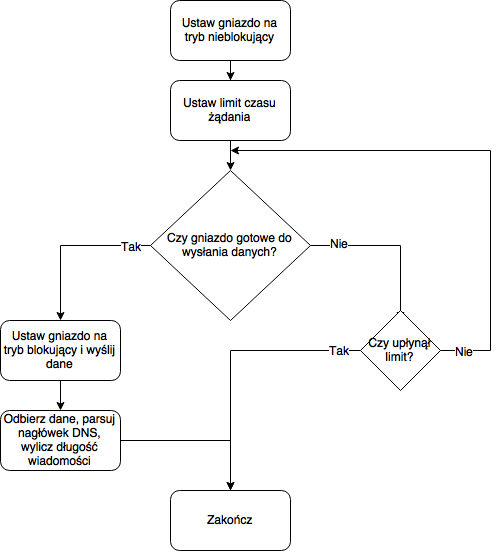
\includegraphics[width=1.0\textwidth]{image/socketAlg}
	\caption{Algorytm dynamicznego ustawiania limitu czasu żądania dla gniazda TCP w blokującym trybie pracy.}
	\label{fig:socketAlg}
\end{figure}

Program umożliwia parsowanie najbardziej popularnych i najczęściej używanych rekordów RR. Zostały one spisane w tabeli \ref{records}
wraz z identyfikatorami, które rezprezentują je w protokole DNS.

\begin{longtable}{|c|c|c|}
	\hline
	\textbf{Lp.} &
	\textbf{Typ rekordu} &
	\textbf{ID rekordu} \\ \hline\hline
	1 & A & 1 \\
	2 & AAAA & 28 \\
    3 & CNAME & 5 \\
	4 & HINFO & 13 \\
	5 & TXT & 16 \\
	6 & NS & 2 \\
	7 & SOA & 6 \\
	8 & PTR & 12 \\
	9 & MX & 15 \\
	10 & RP & 17 \\
	11 & AFSDB & 18 \\
	12 & LOC & 29 \\
	13 & SRV & 33 \\
	14 & NAPTR & 35 \\
	15 & RRSIG & 46 \\
	16 & NSEC & 47 \\
	17 & DNSKEY & 48 \\
	\hline
	\caption{Rekordy DNS obsługiwane w skanerze wraz z identyfikatorami.}
	\label{records}
\end{longtable}

Algorytm postępowania w przypadku odebrania pakietu danych przedstawiony jest na rysunku \ref{fig:receiving}. Dane odbierane z interfejsu
sieciowego są zapisane w systemie szesnastkowym, zgodnie z zaleceniami znanymi dokumentu RFC 1035 \cite{RFC1035}.

\begin{figure}[ht]
	\centering
	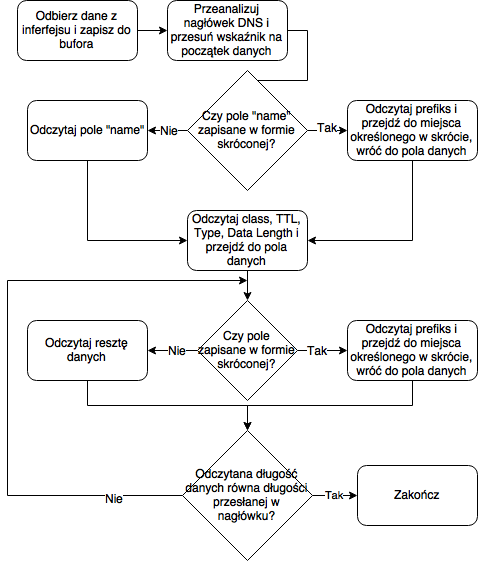
\includegraphics[width=1.0\textwidth]{image/receiving}
	\caption{Algorytm postępowania w przypadku odebrania APDU protokołu DNS.}
	\label{fig:receiving}
\end{figure}

Dodatkowo, jeśli zostanie odebrany typ, który nie został przewidziany w implementacji parsera to wszystkie dane odczytane z
socketa zostaną przeniesione w formie zapisu heksadecymalnego do pliku z odpowiedzią. Zapewnia ta kompatybilność z innymi
rozszerzeniami protokołu DNS oraz zabezpiecza przed błędnym wykluczeniem niektórych informacji ze skanowania. Jeśli pojawi
się nieznany wcześniej typ rekordu z bazy danych DNS, to będzie można interpretować go podczas analizy konkretnych odpowiedzi
od serwera.

Tak jak wcześniej wspomniano, transfer strefy DNS wykorzystuje protokół TCP, który nie jest tak powszechnie stosowany jeśli chodzi
o protokół Doman Name System. Wpływa to pośrednio na to, jakie wyniki możemy uzyskać przy próbie odpytania serwera o jego strefę. Mowa tu o
trzech charakterystycznych sytuacjach, mianowicie:
\begin{enumerate}
	\item brak możliwości nawiązania połączenia na warstwie 4 (TCP) na porcie 53,
	\item uzyskanie połączenia w rozumieniu protokołu TCP na porcie 53 i brak możliwości transferu danych,
	\item uzyskanie połączenia TCP na porcie 53 i pomyślny transfer danych.
\end{enumerate}

Początkowo założono, że uzyskanie już samego połączenia TCP z serwerem może być ciekawym przedmiotem badania. Interfejs serwera
autorytatywnego danej domeny powinien umożliwiać swoim klientom tylko kilka podstawowych operacji, jak na przykład translację nazwy
domenowej komputera ze swojej strefy na jego adres. Do takich działań połączenie TCP nie powinno być potrzebne. Dodatkowo, port 53 na którym działa
DNS jest zarezerwowany tylko dla tego protokołu, więc nie powinno udostępniać się na nim innych usług. Dowodzi to temu, że sytuacja,
gdy możliwe jest nawiązanie połączenia TCP na porcie 53 jest nienaturalna i niezgodna z panującymi dobrymi praktykami. Właśnie dlatego,
w pierwszej implementacji skanera założono, że program będzie tworzył puste pliki w przypadku opisanym w tym akapicie. Niestety,
zjawisko to okazało się tak powszechne, że powstały duże problemy związane z wydajnością skanera. Mowa tu o dostępie poszczególnych
procesów do dysku twardego maszyny na której były one uruchomione. Dlatego też zdecydowano się na zapisywanie informacji jedynie o
domenach, które odpowiedziały na zapytanie AXFR a sytuację umożliwiania nawiązywania sesji TCP na porcie 53 pozostawia się do analizy
podczas przyszłych badań.

Ostatecznie przyjęto rozwiązanie, które ignoruje fakt nawiązywania połączenia TCP oraz odpowiedzi od serwerów, w których nie ma
żadnych rekordów. Pozwoliło to na niemal dwukrotny wzrost wydajności zaimplementowanego skanera.

\section{Dane wejściowe}
\label{inputData}
Dane wejściowe programu zostały pozyskane od grupy naukowców z TU Delft \cite{delft} w formie par (domena, adres IP serwera
autorytarnego). Lista w takim formacie przechowywana była w pliku tekstowym. Zgromadzono w nim, zgodnie z tym co zostało przyjęte
w obliczeniach \ref{obliczenia}, ponad 5 miliardów wpisów uporządkowanych w kolejności alfabetycznej, a ich łączny rozmiar przekraczał
130 gigabajtów. Powoduje to oczywiście szereg problemów związanych z procesowaniem takich plików. (?? skad dane)

Jedną z niedogodności, które wiążą się z rozmiarem danych wejściowych był problem z wyborem losowej próby do kolejnych procesów
skanera. Pożądane jest, aby plik wejściowy do każdego z procesów skanujących nie był w żaden sposób uporządkowany, a najlepiej
gdyby dane w nim zawarte były wybrane losowo. Nie można założyć, że wszystkie procesy skanowania zakończą się bez żadnych błędów.
Jeśli więc dane wejściowe byłyby uporządkowane a proces zakończył się błędem wprowadzona zostanie dodatkowa, błędna korelacja między
brakiem odpowiedzi od serwera a nazwą domeny.

W systemach Linux dostępny jest domyślnie program \textit{shuf} \cite{shuf}, który dokonuje permutacji na konkretnych liniach w pliku,
jednak niemożliwe było wykorzystanie go wraz z plikiem z danymi wejściowymi z powodów ograniczeń wydajnościowych. Program nie był w
stanie zaalokować odpowiedniej liczby komórek w pamięci komputera. Aby zasymulować element losowości zastosowano algorytm zaprezentowany
na diagramie na rysunku \ref{fig:shufAlgorithm} oparty na dzieleniu całego zbioru danych wejściowych oraz permutowaniu kolejnych linii
w podgrupach o różnej wielkości.

\begin{figure}[ht]
	\centering
	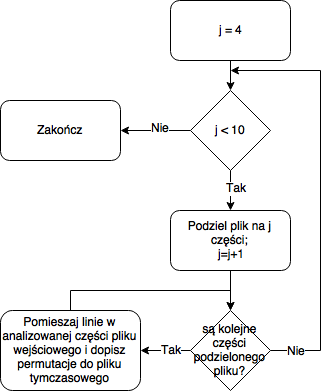
\includegraphics[width=0.6\textwidth]{image/sfuh}
	\caption{Algorytm mieszania linii w dużym pliku wejściowym.}
	\label{fig:shufAlgorithm}
\end{figure}

Następnie, plik został podzielony na mniejsze, po 25000 linii w każdym. Liczba linii w pojedynczym pliku została ustalona arbitralnie,
tak aby widoczny był postęp w skanowaniu. Przeprocesowanie 25 tysięcy linii odpowiada maksymalnie około 28 godzinom przy założeniu,
że dla każdej domeny upłynie limit czasu żądania.

\section{Środowisko uruchomieniowe}
Każda z aplikacji była rozwijana w podobny sposób. Cały proces można podzielić na 3 główne etapy:
\begin{enumerate}
	\item rozwijanie oprogramowania -- dodawanie nowych funkcji do skanera oraz proste testy funkcjonalne,
	\item uruchomienie w warunkach testowych -- sprawdzanie poprawności działania systemu w dłuższej perspektywie (do kilkunastu godzin),
	\item uruchomienie w środowisku docelowym -- właściwe skanowanie maksymalizujące wydajność.
\end{enumerate}
Ze względu na wygodę, każdy z etapów był uruchamiany na innej maszynie. Dostępność sprzętu była ograniczona, dlatego nie udało się
zapewnić, że każda z faz zostanie uruchomiona na takim samym urządzeniu. Faza pierwsza realizowana była na komputerze z procesorem
dwurdzeniowym Intel Core i3-4150, 8GB pamięci RAM oraz 1TB dyskiem twardym w zestawieniu ze 120GB dyskiem SSD. Etap uruchomienia systemu w
środowisku testowym przebiegał na maszynie z procesorem Intel Core2Duo E6420 z dwoma rdzeniami, 4GB pamięci RAM oraz 320GB dyskiem twardym. Etap ostatni,
właściwe skanowanie domen odbywało się na serwerze dedykowanym wypożyczonym od firmy OVH. Zaopatrzony był on w czterordzeniowy
procesor Intel Xeon E3-1230v6, 16GB pamięci RAM oraz 2x4TB dysk twardym.

Każda z maszyn działała pod kontrolą systemu operacyjnego opartego na dystrybucji systemu Debian. Podejście do problemu
w zaprezentowany sposób pozwoliło na szereg udogodnień. Pierwszy etap jest dość oczywisty -- nie ma sensu uruchamiać całego systemu
na serwerze, jeśli nie mamy pewności, że poszczególne komponenty w samym skanerze nie są odpowiednio zaimplementowane. Mylące może
być wprowadzenie etapu uruchomienia systemu w środowisku testowym. Powodem przyjęcia takiego rozwiązania były kwestie finansowe.
Nie mając pewności, że system działa dobrze w długiej perspektywie, nie warto było wypożyczać dedykowanego serwera jedynie do testowania.
W momencie, gdy można było domniemywać, że system działa stabilnie przez dłuższy okres, można było wypożyczyć serwer i skupić się
na uzyskaniu jak największej wydajności skanera.

\section{Metodyka badań}
Skaner został zaprojektowany w takie sposób, aby potrafił przeskanować kilka domen podczas jednego uruchomienia. Założenie wynika z
ograniczeń wydajnościowych, które zauważono przy próbie implementacji skanera, którą opisano w punkcie \ref{dig_sh}.

Skanera nie zaprojektowano tak, aby wspierał wielowątkowość. Może się okazać, że implementacja uruchamiania wielu wątków już w programie
będzie jeszcze bardziej wydajna niż proponowana w niniejszej pracy. Mimo to, opisywana propozycja zakłada realizację wielowątkowości
poprzez uruchomienie wielu procesów programu w systemie linux, każdy z inną listą domen do przeskanowania jako argumentem wejściowym.
Generacja poszczególnych list została opisana we wcześniejszym podpunkcie \ref{inputData}.

Pełen scenariusz skanowania zaprezentowano poniżej.
\begin{enumerate}
	\item Pobierz listę do skanowania.
	\item Wygeneruj N podzbiorów rozłącznych dla listy.
	\item Dla każdego podzbioru uruchom proces skanera z odpowiadającą mu listą.
\end{enumerate}

W prezentowanym przypadku liczba podzbiorów była bardzo duża, więc zdecydowano się na ograniczenie liczby uruchamianych procesów
skanera jednocześnie. Eksperymentalnie ustalono, że liczba instancji skanera na poziomie 15000 jest akceptowalna zarówno ze względu
na wydajność jak i stabilność. Ustalone ograniczenie zostało zrealizowane dzięki skryptom powłoki bash -- cyklicznie sprawdzano ile
uruchomionych jest aktualnie instancji skanera, jeśli liczba była mniejsza od 15000, to uruchamiano procesy w liczbie takiej,
aby suma uruchomionych procesów skanera osiągała liczbę 15000. Aby uniknąć konfliktów zapisu do plików ustalono, że każdy z uruchomionych
procesów będzie zapisywał odebrane informacje do oddzielnych katalogów. Katalogi były indeksowane, ich nazwa byla postaci
,,iter\_{numer\_iteracji}''. Umożliwioło to wyeliminowanie dzielenia zasobów pomiędzy procesami, co przełożyło się na wydajność całego
rozwiązania.


\section{System powiadomień}
W ramach badań przeprowadzonych podczas realizacji niniejszej pracy magisterskiej został zaimplementowany i uruchomiony system
powiadamiania administratorów domen. System bazuje na informacjach pobranych podczas skanowania podatności serwerów na zapytania
typu AXFR. W rekordzie SOA przesyłanym na początku i na końcu wiadomości przesyłany jest adres osoby odpowiedzialnej za daną domenę.
Jego miejscem jest pozycja numer 2. w rekordzie SOA z tą różnicą, że pierwszy znak ,,.'' napotkany w adresie jest zamieniany na
znak ,,@''. W wyniku tej zamiany uzyskiwany jest adres mailowy, przypisany do administratora domeny.

System powiadomień zaimplementowano w systemie operacyjnym z rodziny systemów UNIX. Opiera się on głównie na skryptach powłoki
\textit{bash}. Algorytm wyodrębnia rekordy SOA i wypisuje je do pliku. Następnie plik sortowany jest ze względu na adres mailowy
administratora domeny, po czym grupuje się te domeny, za które odpowiada ten sam adres pocztowy. Kolejnym krokiem jest pogrupowanie
domen oraz utworzenie odpowiedniego pliku tekstowego. Zawarte są w nim domeny oraz adresy serwerów które umożliwiają transfer
strefy dla danej domeny. Nazwa pliku odpowiada adresowi mailowemu zarządcy domeny.

Po otrzymaniu zbioru plików opisanych powyżej uruchamiany jest proces, którego zadaniem jest wysłanie wiadomości pod określone
adresy. Skrypt, który automatyzuje opisaną czynność napisano w języku Python \cite{python}. Wysyłane wiadomości podpisywane są
kluczem PGP \cite{RFC4880}, aby odbiorca mógł zweryfikować, że wiadomość została odebrana dokładnie w takiej formie jak ją przygotowano
i wysłano.


\chapter{Obserwacje i wyniki}
Przeprocesowanie dostarczonego zbioru danych zajęło 11 dni, co poskutkowało zebraniem około 30GB informacji na temat analizowanych domen.

\section{Typy odebranych odpowiedzi}
Wśród przeanalizowanych par domen i serwerów można zaobserwować kilka charakterystycznych typów odpowiedzi. Odpowiedzi mogą być dzielone na kategorie ze względu na różne kryteria. Pierwszym kryterium, które będzie brane pod uwagę w niniejszej pracy jest po prostu rozmiar pliku przechowującego informacje pobrane z serwera autorytatywnego. Jest to motywowane faktem, że w istocie im większy jest plik z odpowiedzią, tym spodziewamy się, że zawiera on więcej informacji na temat odpytywanej domeny. 

Pierwszym typem jest odpowiedź, która zajmowała na dysku specyficzną ilość miejsca -- 25123 bajty. Zaobserwowano, że uzyskano 626288 odpowiedzi tego typu. Rozmiar pliku jest swego rodzaju skutkiem ubocznym uproszczonej implementacji skanera. Trudno było przewidzieć wszystkie specyficzne przypadki towarzyszące transferowi strefy DNS. Zaobserwowana sytuacja jest właśnie jednym z tych nietypowych sytuacji i nawet program dig nie odwzorowuje idealnie zachowania jakie powinno nastąpić w takiej sytuacji. przyczyna utworzenia opisanego wcześniej pliku nie jest jednoznacznie określona. Zostały podjęte próby ustalenia czym spowodowane jest takie zachowanie. W takich samych przypadkach program dig zwraca jedynie rekord DNS SOA i komunikat o błędzie (ang. \textit{communications error: end of file}). Zachowanie programu dig w dużym stopniu przypomina przekierowanie zapytania IXFR na AXFR (ang. \textit{AXFR fallback}) opisane między innymi w RFC1995\cite{RFC1995}. Wywołanie mechanizmu AXFR fallback następuje w sytuacji, kiedy numer wersji pliku strefy przysłany do serwera jest wyższy niż numer wersji aktualnie na nim przechowywany. Na różnego rodzaju forach\cite{powerdns-forum} czy w serwisach internetowych\cite{powerdns-git}, problem który został opisany pojawia się najczęściej jako problem implementacji oprogramowania PowerDNS\cite{powerdns}. Niemniej jednak nie ustalono dokładnie jaki jest powód wysłania tak dużego pakietu w odpowiedzi na zwykłe zapytanie AXFR.

Kolejnym przykładem odpowiedzi, która powodowała powstanie dużego pliku na dysku, było odebranie od serwera autorytatywnego pakietu TCP RST(ang. \textit{TCP reset packet}). Sytuacja taka wynika również z pewnego uproszczenia, które zostało przyjęte w implementacji skanera. Założono, że zawsze zostanie odebrany pakiet DNS. Podyktowane było to ograniczonym czasem w którym implementowano skaner oraz faktem, że problem ten można w łatwy sposób obejść poprzez odfiltrowanie odpowiednich plików w katalogu z wynikami. Dodatkowo sytuacje tego typu były bardzo sporadyczne, więc nie afektowało to w znaczącym stopniu ani na czas przeanalizowania pobranych danych ani na wynik tej analizy.

Kolejnymi specyficznymi grupami jeśli chodzi o rozmiar pliku z odpowiedzią są już typowe odpowiedzi na zapytania AXFR. Najmniejszy rozmiar mają oczywiście odpowiedzi, które zawierają jedynie rekord SOA i jest to dopuszczalna odpowiedź na zapytanie AXFR. Następnie, wraz ze zwiększającą się liczbą wpisów w pliku strefy DNS, zwiększa się rozmiar odpowiedzi. Nie przekłada się to jednak bezpośrednio na informacje, które można wyodrębnić z takich plików strefy. Zdarza się bowiem sytuacja, w której znaczną część pliku strefy DNS zajmują wpisy podpisów cyfrowych RRSIG, których długość przekłada się na rozmiar plików. Dodatkowo, podpisy generowane mogą być dla każdego rekordu oddzielnie (co szerzej opisano w podpunkcie \ref{RSIG}), dlatego też wpływa to bardzo znacząco na rozmiar otrzymywanej odpowiedzi.

\section{Odebrane adresy IPv4}
Częstym argumentem, który pojawia się podczas dyskusji na temat bezpieczeństwa transferów plików bazy danych DNS jest ujawnianie adresów IP. W niniejszym podrozdziale skupiono się głównie na adresach IP w wersji 4. ponieważ jest to wciąż dominujący typ adresacji w Internecie. Okazuje się, że pomimo obaw o wycieki adresów przez dokonywanie nieuprawnionego transferu nikt nie zbadał dokładnie jak duża może być skala tego zjawiska. Umożliwiły to badania przeprowadzone w tej pracy magisterskiej.

Po przeprowadzeniu skanowania okazało się, że dzięki przeprowadzonemu skanowaniu uzyskano informację o ponad <123456789> publicznych adresach IP w wersji 4. 

\section{Analiza TLD}
Jednym z podejść analizy zebranego zbioru danych było sprawdzenie, jak przedstawia się rozkład popularności domeny najwyższego poziomu dla serwerów podatnych na nieuprawiony transfer strefy. 

W głównej mierze należy zastanowić się, czy rozkład ten jest w ogóle istotny, czy może nie różni się on niczym od ogólnego, całościowego rozkładu popularności TLD w internecie, bez uwzględnienia podatności czy innych czynników. W tym celu przeanalizowano i przedstawiono wykres popularności domen najwyższego poziomu w sieci internet. Jest on przedstawiony na rysunku \ref{TLD_all}.
\begin{center}
	\begin{figure}
		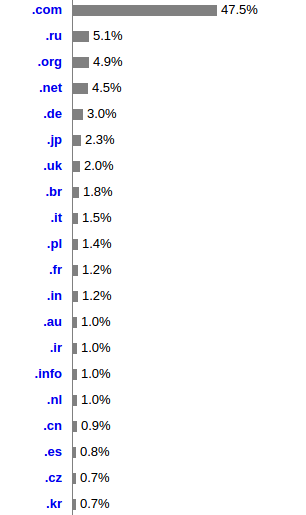
\includegraphics[scale=0.75]{image/TLD_all}\label{TLD_all}
		\caption{Popularność TLD w internecie (dostęp na dzień 15. maja 2017), źródło:  \cite{TLD_popularity}}
	\end{figure}
\end{center}  

Wykres przedstawia procentowy rozkład poszczególnych domen internetowych w zależności od używanej domeny najwyższego poziomu. Wynika z niego, że domena najwyższego poziomu \textit{.com} jest używana przez 47.5\% wszystkich domen. Wykres ograniczony został do 20 najbardziej popularnych TLD. Różnice pomiędzy kolejnymi rekordami są na tyle niskie, że ich umieszczenie wpływałoby negatywnie na ogólną reprezentację wyników. Wykres \ref{TLD_all} zostanie następnie zestawiony z popularnością TLD tych domen, których serwery autorytatywne umożliwiają nieuprawniony transfer AXFR. Rozkład popularności TLD domen odpowiadających na zapytanie AXFR przedstawiono na rysunku \ref{resp}.
\begin{center}
	\begin{figure}
		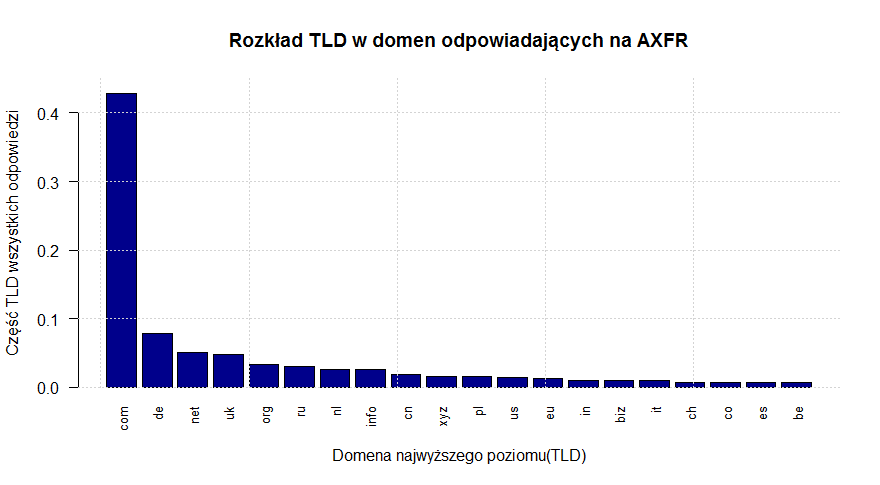
\includegraphics[width=1.0\textwidth]{image/resp}\label{resp}
		\caption{Popularność TLD w odpowiedziach AXFR.}
	\end{figure}
\end{center} 

Dokonując porównania wykresów \ref{TLD_all} oraz \ref{resp} możemy dostrzec kilka prawidłowości. Zarówno w jednym jak i drugim przypadku, wyraźnie dominującą domeną najwyższego poziomu jest domena .com. Dodatkowo, nie można mówić tu o anomalii, ponieważ zarówno w jednym jak i drugim przypadku domena .com stanowi bardzo podobny procentowy udział wszystkich domen, czy to pytanych czy tych, które odpowiedziały. Następnie można dostrzec delikatne zmiany w procentowych udziałach kolejnych TLD, jednak nie na pierwszy rzut oka zmiany te nie są wyróżniające się czy nad wyraz zauważalne.

W związku z tym, że wyżej opisane działania nie pozwoliły na wyraźne zarysowanie różnic pomiędzy rozkładami TLD, zdecydowano się zestawić ze sobą inne zbiory danych. Wykreślono podobne wykresy dla popularności domeny najwyższego poziomu dla domen odpytywanych podczas skanowania oraz TLD domen, które na zapytania odpowiedziały. Następnie zestawiono ze sobą wyniki pozyskane z obu tych zbiorów danych. Zostały odpowiednio wykreślone:
\begin{enumerate}
	\item wykres 15 najpopularniejszych TLD w zbiorze domen odpytywanych w porównaniu do popularności tych TLD w zbiorze domen które odpowiedziały na zapytanie AXFR -- wykres \ref{req_to_resp},
	\item wykres 15 najpopularniejszych TLD w zbiorze domen które odpowiedziały na zapytanie AXFR w zestawieniu z ich popularnością w puli TLD domen odpytywanych -- wykres \ref{resp_to_req}.
\end{enumerate}

\begin{figure}[ht]
	\centering
	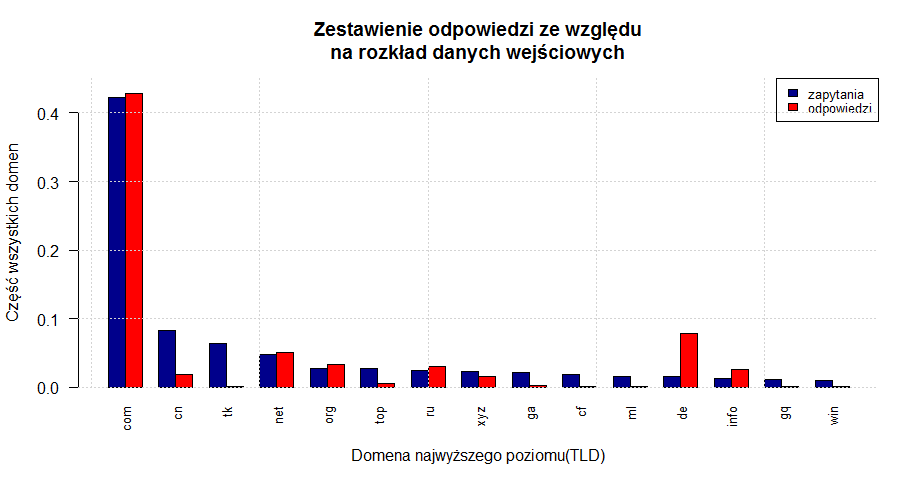
\includegraphics[width=1.0\textwidth]{image/req_to_resp}
	\caption{}
	\label{req_to_resp}
\end{figure}

\begin{figure}[ht]
	\centering
	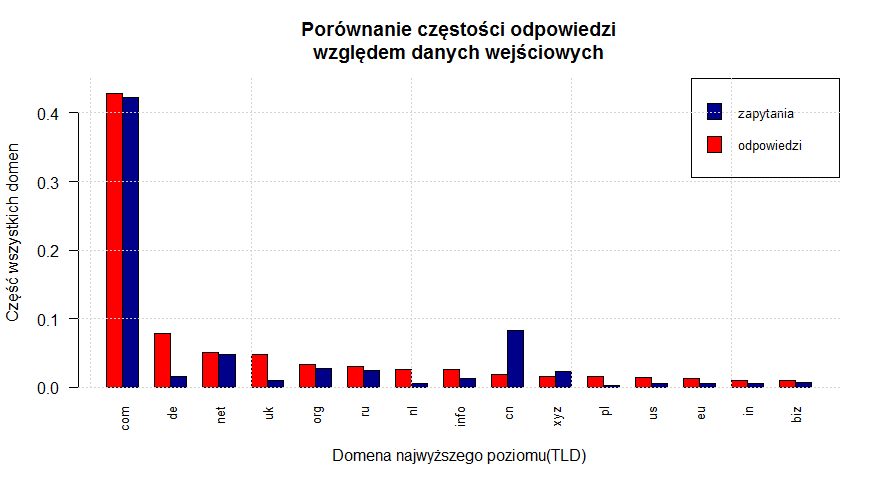
\includegraphics[width=1.0\textwidth]{image/resp_to_req}
	\caption{}
	\label{resp_to_req}
\end{figure}

W przypadku tych bezpośrednich zestawień, można zauważyć więcej interesujących prawidłowości. Na początku warto wspomnieć, że istnieje duża dysproporcja w przypadku niektórych domen najwyższego poziomu. Pierwszą z nich może być przypadek domeny .de, gdzie procentowy udział TLD .de we wszystkich TLD odpowiedzi AXFR jest drugim wynikiem podczas gdy w populacji danych wejściowych jest to 12 najliczniejsza grupa. Warto dodać, że domena .de jest jedną z domen, których zarządcy traktują proceder \textit{zone enumeration} jako łamanie prawa, co opisano w podpunkcie \ref{zone_enumeration}. Transfer AXFR pozwala na uzyskanie danych o podobnej charakterystyce, a mimo to, ok 8\% wszystkich odpowiedzi powiązane jest z domeną najwyższego poziomu .de (domena regionalna -- Niemcy). Podobna sytuacja ma miejsce również w przypadku TLD .uk (Wielka Brytania) czy .pl (Polska), gdzie przy małym współczynniku domen odpytywanych otrzymano nieproporcjonalnie wysoki współczynnik odpowiedzi.

Zjawiskiem w pewnym stopniu odwrotnym do opisanego w poprzednim akapicie jest rozkład zapytań/odpowiedzi dla TLD .cn (Chiny) lub .tk (Tokelau -- region zależny od Nowej Zelandii). W tym przypadku zauważalna jest również duża dysproporcja, jednak ,,na korzyść'', gdyż w stosunku do wielu zapytań wystosowanych do domen należących do tych TLD uzyskano relatywnie mało odpowiedzi. Dodatkowo, do grupy opisywanej w tym akapicie można zaliczyć również TLD .top, która została oficjalnie wydzielona w 2014 roku. (... ?)

Oprócz opisanych wcześniej względnych porównań pomiędzy pytaniami i odpowiedziami od serwerów autorytatywnych różnych domen sprawdzono jak wygląda dystrybuanta poszczególnych rozkładów. Pozwoliło to oszacować ile (ilościowo) domen najwyższego poziomu zawierało się w grupie, dla której generowano większość zapytań (rysunek \ref{cdf_tld_req}). Analogicznie, w przypadku danych dotyczących odpowiedzi AXFR można było ocenić ile różnych TLD pojawia się niemal we wszystkich odpowiedziach (rysunek \ref{cdf_tld_resp}).

\begin{figure}[ht]
	\centering
	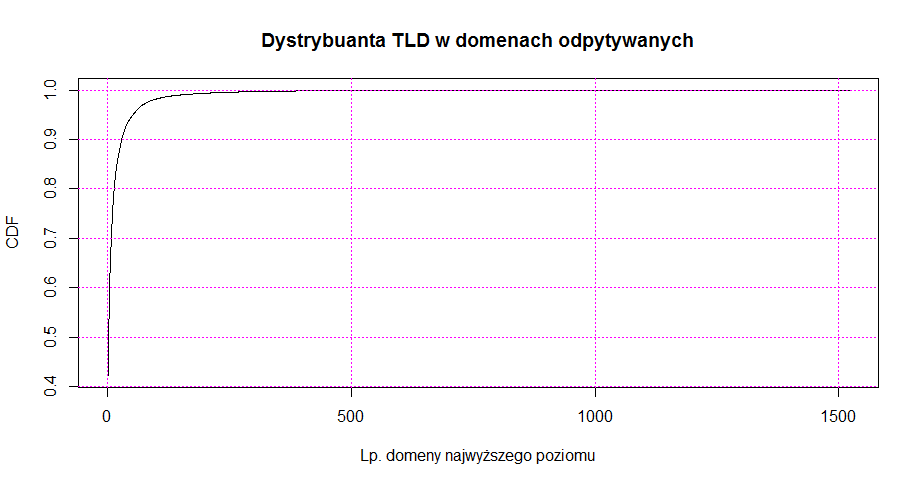
\includegraphics[width=1.0\textwidth]{image/cdf_tld_req}
	\caption{}
	\label{cdf_tld_req}
\end{figure}

\begin{figure}[ht]
	\centering
	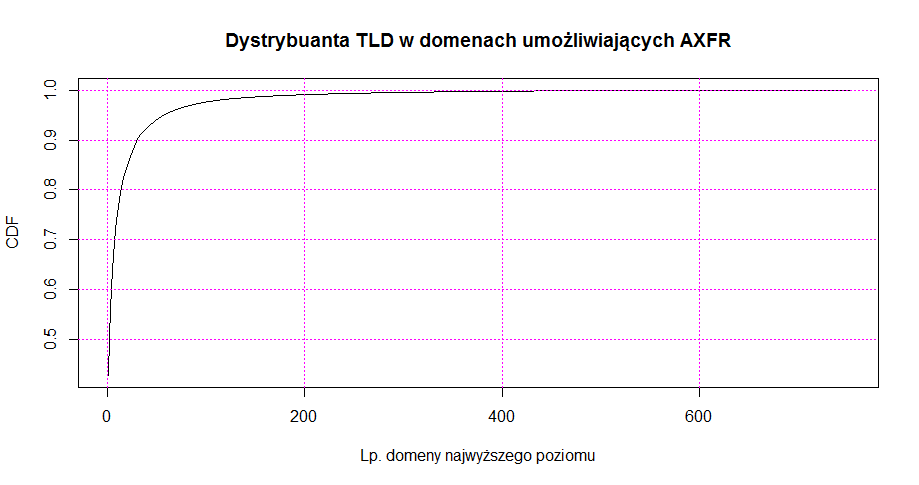
\includegraphics[width=1.0\textwidth]{image/cdf_tld_resp}
	\caption{}
	\label{cdf_tld_resp}
\end{figure}

\begin{table}[]
	\centering
	\caption{Opis zbiorów zapytań/odpowiedzi}
	\label{cdf_table}
	\begin{tabular}{|p{0.2\textwidth}|p{0.3\textwidth}|p{0.4\textwidth}|}
		\hline
		\textbf{Zbiór} & 
		\textbf{Liczba różnych TLD w zbiorze} & 
		\textbf{Liczba różnych TLD zawierająca 99\% elementów zbioru} \\
		\hline\hline
		Zapytania & 
		1521 & 
		147\\
		\hline
		Odpowiedzi & 
		751 & 
		187\\
		\hline\hline		
	\end{tabular}
\end{table}

Oprócz wykreślonych charakterystyk policzono również ile domen najwyższego poziomu gromadzi w sobie 99\% zapytań bądź odpowiedzi (w zależności od badanego zbioru). Wyniki zaprezentowano w tabeli \ref{cdf_table}. Warto zauważyć, że pomimo ponad dwukrotnie mniejszego zbioru różnych domen poziomu najwyższego, należy zgrupować dużo więcej TLD aby uzyskać zbiór 99\% wszystkich odpowiedzi. Można z tego wnioskować, że rozkład odpowiedzi jest bardziej jednostajny niż w przypadku danych wejściowych. Można także przypuszczać, że zbiór wejściowy zawierał pojedyncze domeny z różnych, rzadko spotykanych TLD. W momencie, kiedy jedna, czy jedynie kilka domen z takiego TLD są odpowiednio zabezpieczone przed nieuprawnionym transferem AXFR nie znajdziemy danego sufiksu w zbiorze odpowiedzi. Sytuacja taka może mieć miejsce, gdy wszystkie domeny z mało popularnego TLD znajdują się pod zarządem jednej osoby czy organizacji.


\section{Analiza AS}
Podstawową informacją, którą uzyskać można wykorzystując pobrane dane z transferów AXFR jest przynależność otrzymanych adresów IP do konkretnych grup autonomicznych. Grupy te określają przynależność do sieci, które zarządzane są przed tego samego operatora sieciowego, a wykorzystuje się je głównie w protokołach routingu. Informacje związane z systemami autonomicznymi można, w głównej mierze, znaleźć w RFC1930\cite{RFC1930}.


\chapter{Podsumowanie}
\noindent W niniejszej pracy magisterskiej zaproponowano unikatowe podejście do problemu transferu strefy AXFR oparte na globalnym skanowaniu
domen i ich serwerów przestrzeni nazw. Przeanalizowano, czy powszechnie dostępne narzędzia zapewniają takie funkcje, aby przeprowadzić
badania w zakresie postawionego problemu. Została zaproponowana implementacja oraz wdrożenie systemu, który umożliwia optymalne wykonanie
takich badań. Zebrano oraz przeanalizowano dane, które można uzyskać w wyniku globalnego skanowania domen pod kątem podatności
na transfer AXFR. Pogrupowano uzyskane odpowiedzi, typy zachowań na wystosowane żądanie AXFR. Opisano, w jaki sposób mogą odpowiadać
serwery autorytatywne oraz przeanalizowano popularność każdego z typów otrzymywanej odpowiedzi.

Podsumowując przeprowadzone prace i badania okazuje się, że transfer strefy wykorzystując mechanizm AXFR jest wciąż możliwy dla
bardzo wielu domen. Bardzo duża część domen jest pod zarządem niewielkiej liczby serwerów autorytatywnych, więc możliwe, że zezwolenie
na taki transfer bywa zamierzone. Resztę można zaliczyć jako niepoprawnie skonfigurowane i to one są najbardziej narażone na
ataki cyberprzestępców. Zalecenia wydane w dalszej części rozdziału są kierowane głównie w kierunku administratorów właśnie tych domen.

W pracy opisano także, które części stref DNS pozwalają cyberprzestępcom na pozyskanie informacji na temat ich potencjalnych celów.
Skupiono się w głównej mierze na usługach uruchamianych w badanych systemach, informacjach na temat infrastruktury antyspamowej,
ale także na pośrednim wykorzystaniu danych maszyn w innych typach ataków.

\section{Zalecenia}
\noindent Transfer strefy AXFR pozwala na uzyskanie wielu informacji na temat tego, jakie usługi oraz jakie maszyny są uruchomione wewnątrz danej
domeny. Drastycznym, ale najbardziej skutecznym zaleceniem jest wycofanie z implementacji serwerów DNS funkcji transferu strefy DNS do
każdej maszyny wystosowującej zapytanie tego typu. Wymagałoby to używania jedynie adresów IP serwerów, które mogą ten transfer przeprowadzić.
Rozwiązanie to ograniczyłoby skalowalność rozwiązania, jednak jawne podanie adresu IP jest dużo bardziej bezpieczne i zapewnia, że
transfer strefy przeprowadzony będzie tylko przez te maszyny, którym rzeczywiście, wprost, na to zezwolono.

Innym rozwiązaniem jest rezygnacja z własnych serwerów DNS na rzecz usług \textit{DNS as a service} (rozdział \ref{dnsasservice}). Takie postępowanie eliminuje większość
problemów związanych z transferem strefy, gdyż cała infrastruktura jest dzierżawiona od zewnętrznej firmy. Firmom takim również zależy
na jak najlepszej jakości ich usług oraz zależy im, aby dane na temat stref DNS nie były tak powszechnie dostępne, dlatego dobrze
zabezpieczają transfer strefy. Odbywa się to na przykład dzięki zestawieniu sesji SSL pomiędzy stronami wymieniającymi dane, bądź
innym wykorzystaniu kryptografii (na przykład szyfrowanie).

\section{Retrospekcja}
\noindent Pośrednim wynikiem tworzenia niniejszej pracy magisterskiej mogą być również wnioski na temat samego procesu jej realizacji czy przeprowadzania badań.
Nie wszystkie etapy pracy były przeprowadzane płynnie, co pozwala na wyciągnięcie wniosków pozwalających uniknąć takich sytuacji
w przyszłości. Jednym z trudniejszych etapów realizacji pracy było przygotowanie oprogramowania i środowiska pod globalne skanowanie.
Trud ten wynika głównie ze skali, skrypty dostępne w Internecie nie są aż tak wydajne aby zapewnić oczekiwaną wydajność. Poważnym
błędem, który spowodował wydłużenie czasu uruchomienia systemu były próby wykorzystania już istniejących narzędzi, jednak pozwoliło to
na opisanie ich wad bądź zalet. Dodatkowo, można wyciągnąć wniosek, że przeprowadzanie skanowania na szeroką skalę bardzo często wymaga
implementacji oprogramowania dokładnie pod kątem tego specyficznego przypadku, bardzo często bez używania innych projektów powiązanych
z tematyką badań. Oprogramowanie skanera jest ciągle ulepszane, co dowodzi temu, że nawet kilka miesięcy działania systemu nie pozwala
na pełne, dokładne przetestowanie skanera.


\bibliography{bibliography}
\nocite{*}
\bibliographystyle{plain}
\listoffigures
\listoftables

\end{document}
